\documentclass[journal]{IEEEtran}
%
% If IEEEtran.cls has not been installed into the LaTeX system files,
% manually specify the path to it like:
% \documentclass[journal]{../sty/IEEEtran}





% Some very useful LaTeX packages include:
% (uncomment the ones you want to load)
\usepackage[spanish]{babel}
\usepackage[utf8]{inputenc}
\usepackage{url}
\usepackage{minted}
\setminted{fontsize=\small,baselinestretch=1}
\usepackage{listings}
\usepackage{subcaption}
\renewcommand\listingscaption{Código}
\newenvironment{code}{\captionsetup{type=listing}}{\par\addvspace{\baselineskip}}
\usepackage{graphicx}
\usepackage{tikz}
\usetikzlibrary{scopes}
\usetikzlibrary{babel}

% *** MISC UTILITY PACKAGES ***
%
%\usepackage{ifpdf}
% Heiko Oberdiek's ifpdf.sty is very useful if you need conditional
% compilation based on whether the output is pdf or dvi.
% usage:
% \ifpdf
%   % pdf code
% \else
%   % dvi code
% \fi
% The latest version of ifpdf.sty can be obtained from:
% http://www.ctan.org/pkg/ifpdf
% Also, note that IEEEtran.cls V1.7 and later provides a builtin
% \ifCLASSINFOpdf conditional that works the same way.
% When switching from latex to pdflatex and vice-versa, the compiler may
% have to be run twice to clear warning/error messages.






% *** CITATION PACKAGES ***
%
%\usepackage{cite}
% cite.sty was written by Donald Arseneau
% V1.6 and later of IEEEtran pre-defines the format of the cite.sty package
% \cite{} output to follow that of the IEEE. Loading the cite package will
% result in citation numbers being automatically sorted and properly
% "compressed/ranged". e.g., [1], [9], [2], [7], [5], [6] without using
% cite.sty will become [1], [2], [5]--[7], [9] using cite.sty. cite.sty's
% \cite will automatically add leading space, if needed. Use cite.sty's
% noadjust option (cite.sty V3.8 and later) if you want to turn this off
% such as if a citation ever needs to be enclosed in parenthesis.
% cite.sty is already installed on most LaTeX systems. Be sure and use
% version 5.0 (2009-03-20) and later if using hyperref.sty.
% The latest version can be obtained at:
% http://www.ctan.org/pkg/cite
% The documentation is contained in the cite.sty file itself.






% *** GRAPHICS RELATED PACKAGES ***
%
\ifCLASSINFOpdf
  % \usepackage[pdftex]{graphicx}
  % declare the path(s) where your graphic files are
  % \graphicspath{{../pdf/}{../jpeg/}}
  % and their extensions so you won't have to specify these with
  % every instance of \includegraphics
  % \DeclareGraphicsExtensions{.pdf,.jpeg,.png}
\else
  % or other class option (dvipsone, dvipdf, if not using dvips). graphicx
  % will default to the driver specified in the system graphics.cfg if no
  % driver is specified.
  % \usepackage[dvips]{graphicx}
  % declare the path(s) where your graphic files are
  % \graphicspath{{../eps/}}
  % and their extensions so you won't have to specify these with
  % every instance of \includegraphics
  % \DeclareGraphicsExtensions{.eps}
\fi
% graphicx was written by David Carlisle and Sebastian Rahtz. It is
% required if you want graphics, photos, etc. graphicx.sty is already
% installed on most LaTeX systems. The latest version and documentation
% can be obtained at: 
% http://www.ctan.org/pkg/graphicx
% Another good source of documentation is "Using Imported Graphics in
% LaTeX2e" by Keith Reckdahl which can be found at:
% http://www.ctan.org/pkg/epslatex
%
% latex, and pdflatex in dvi mode, support graphics in encapsulated
% postscript (.eps) format. pdflatex in pdf mode supports graphics
% in .pdf, .jpeg, .png and .mps (metapost) formats. Users should ensure
% that all non-photo figures use a vector format (.eps, .pdf, .mps) and
% not a bitmapped formats (.jpeg, .png). The IEEE frowns on bitmapped formats
% which can result in "jaggedy"/blurry rendering of lines and letters as
% well as large increases in file sizes.
%
% You can find documentation about the pdfTeX application at:
% http://www.tug.org/applications/pdftex





% *** MATH PACKAGES ***
%
%\usepackage{amsmath}
% A popular package from the American Mathematical Society that provides
% many useful and powerful commands for dealing with mathematics.
%
% Note that the amsmath package sets \interdisplaylinepenalty to 10000
% thus preventing page breaks from occurring within multiline equations. Use:
%\interdisplaylinepenalty=2500
% after loading amsmath to restore such page breaks as IEEEtran.cls normally
% does. amsmath.sty is already installed on most LaTeX systems. The latest
% version and documentation can be obtained at:
% http://www.ctan.org/pkg/amsmath





% *** SPECIALIZED LIST PACKAGES ***
%
%\usepackage{algorithmic}
% algorithmic.sty was written by Peter Williams and Rogerio Brito.
% This package provides an algorithmic environment fo describing algorithms.
% You can use the algorithmic environment in-text or within a figure
% environment to provide for a floating algorithm. Do NOT use the algorithm
% floating environment provided by algorithm.sty (by the same authors) or
% algorithm2e.sty (by Christophe Fiorio) as the IEEE does not use dedicated
% algorithm float types and packages that provide these will not provide
% correct IEEE style captions. The latest version and documentation of
% algorithmic.sty can be obtained at:
% http://www.ctan.org/pkg/algorithms
% Also of interest may be the (relatively newer and more customizable)
% algorithmicx.sty package by Szasz Janos:
% http://www.ctan.org/pkg/algorithmicx




% *** ALIGNMENT PACKAGES ***
%
%\usepackage{array}
% Frank Mittelbach's and David Carlisle's array.sty patches and improves
% the standard LaTeX2e array and tabular environments to provide better
% appearance and additional user controls. As the default LaTeX2e table
% generation code is lacking to the point of almost being broken with
% respect to the quality of the end results, all users are strongly
% advised to use an enhanced (at the very least that provided by array.sty)
% set of table tools. array.sty is already installed on most systems. The
% latest version and documentation can be obtained at:
% http://www.ctan.org/pkg/array


% IEEEtran contains the IEEEeqnarray family of commands that can be used to
% generate multiline equations as well as matrices, tables, etc., of high
% quality.




% *** SUBFIGURE PACKAGES ***
%\ifCLASSOPTIONcompsoc
%  \usepackage[caption=false,font=normalsize,labelfont=sf,textfont=sf]{subfig}
%\else
%  \usepackage[caption=false,font=footnotesize]{subfig}
%\fi
% subfig.sty, written by Steven Douglas Cochran, is the modern replacement
% for subfigure.sty, the latter of which is no longer maintained and is
% incompatible with some LaTeX packages including fixltx2e. However,
% subfig.sty requires and automatically loads Axel Sommerfeldt's caption.sty
% which will override IEEEtran.cls' handling of captions and this will result
% in non-IEEE style figure/table captions. To prevent this problem, be sure
% and invoke subfig.sty's "caption=false" package option (available since
% subfig.sty version 1.3, 2005/06/28) as this is will preserve IEEEtran.cls
% handling of captions.
% Note that the Computer Society format requires a larger sans serif font
% than the serif footnote size font used in traditional IEEE formatting
% and thus the need to invoke different subfig.sty package options depending
% on whether compsoc mode has been enabled.
%
% The latest version and documentation of subfig.sty can be obtained at:
% http://www.ctan.org/pkg/subfig




% *** FLOAT PACKAGES ***
%
%\usepackage{fixltx2e}
% fixltx2e, the successor to the earlier fix2col.sty, was written by
% Frank Mittelbach and David Carlisle. This package corrects a few problems
% in the LaTeX2e kernel, the most notable of which is that in current
% LaTeX2e releases, the ordering of single and double column floats is not
% guaranteed to be preserved. Thus, an unpatched LaTeX2e can allow a
% single column figure to be placed prior to an earlier double column
% figure.
% Be aware that LaTeX2e kernels dated 2015 and later have fixltx2e.sty's
% corrections already built into the system in which case a warning will
% be issued if an attempt is made to load fixltx2e.sty as it is no longer
% needed.
% The latest version and documentation can be found at:
% http://www.ctan.org/pkg/fixltx2e


%\usepackage{stfloats}
% stfloats.sty was written by Sigitas Tolusis. This package gives LaTeX2e
% the ability to do double column floats at the bottom of the page as well
% as the top. (e.g., "\begin{figure*}[!b]" is not normally possible in
% LaTeX2e). It also provides a command:
%\fnbelowfloat
% to enable the placement of footnotes below bottom floats (the standard
% LaTeX2e kernel puts them above bottom floats). This is an invasive package
% which rewrites many portions of the LaTeX2e float routines. It may not work
% with other packages that modify the LaTeX2e float routines. The latest
% version and documentation can be obtained at:
% http://www.ctan.org/pkg/stfloats
% Do not use the stfloats baselinefloat ability as the IEEE does not allow
% \baselineskip to stretch. Authors submitting work to the IEEE should note
% that the IEEE rarely uses double column equations and that authors should try
% to avoid such use. Do not be tempted to use the cuted.sty or midfloat.sty
% packages (also by Sigitas Tolusis) as the IEEE does not format its papers in
% such ways.
% Do not attempt to use stfloats with fixltx2e as they are incompatible.
% Instead, use Morten Hogholm'a dblfloatfix which combines the features
% of both fixltx2e and stfloats:
%
% \usepackage{dblfloatfix}
% The latest version can be found at:
% http://www.ctan.org/pkg/dblfloatfix




%\ifCLASSOPTIONcaptionsoff
%  \usepackage[nomarkers]{endfloat}
% \let\MYoriglatexcaption\caption
% \renewcommand{\caption}[2][\relax]{\MYoriglatexcaption[#2]{#2}}
%\fi
% endfloat.sty was written by James Darrell McCauley, Jeff Goldberg and 
% Axel Sommerfeldt. This package may be useful when used in conjunction with 
% IEEEtran.cls'  captionsoff option. Some IEEE journals/societies require that
% submissions have lists of figures/tables at the end of the paper and that
% figures/tables without any captions are placed on a page by themselves at
% the end of the document. If needed, the draftcls IEEEtran class option or
% \CLASSINPUTbaselinestretch interface can be used to increase the line
% spacing as well. Be sure and use the nomarkers option of endfloat to
% prevent endfloat from "marking" where the figures would have been placed
% in the text. The two hack lines of code above are a slight modification of
% that suggested by in the endfloat docs (section 8.4.1) to ensure that
% the full captions always appear in the list of figures/tables - even if
% the user used the short optional argument of \caption[]{}.
% IEEE papers do not typically make use of \caption[]'s optional argument,
% so this should not be an issue. A similar trick can be used to disable
% captions of packages such as subfig.sty that lack options to turn off
% the subcaptions:
% For subfig.sty:
% \let\MYorigsubfloat\subfloat
% \renewcommand{\subfloat}[2][\relax]{\MYorigsubfloat[]{#2}}
% However, the above trick will not work if both optional arguments of
% the \subfloat command are used. Furthermore, there needs to be a
% description of each subfigure *somewhere* and endfloat does not add
% subfigure captions to its list of figures. Thus, the best approach is to
% avoid the use of subfigure captions (many IEEE journals avoid them anyway)
% and instead reference/explain all the subfigures within the main caption.
% The latest version of endfloat.sty and its documentation can obtained at:
% http://www.ctan.org/pkg/endfloat
%
% The IEEEtran \ifCLASSOPTIONcaptionsoff conditional can also be used
% later in the document, say, to conditionally put the References on a 
% page by themselves.

% *** PDF, URL AND HYPERLINK PACKAGES ***
%
%\usepackage{url}
% url.sty was written by Donald Arseneau. It provides better support for
% handling and breaking URLs. url.sty is already installed on most LaTeX
% systems. The latest version and documentation can be obtained at:
% http://www.ctan.org/pkg/url
% Basically, \url{my_url_here}.


% *** Do not adjust lengths that control margins, column widths, etc. ***
% *** Do not use packages that alter fonts (such as pslatex).         ***
% There should be no need to do such things with IEEEtran.cls V1.6 and later.
% (Unless specifically asked to do so by the journal or conference you plan
% to submit to, of course. )


% correct bad hyphenation here
\hyphenation{op-tical net-works semi-conduc-tor}


\begin{document}
%
% paper title
% Titles are generally capitalized except for words such as a, an, and, as,
% at, but, by, for, in, nor, of, on, or, the, to and up, which are usually
% not capitalized unless they are the first or last word of the title.
% Linebreaks \\ can be used within to get better formatting as desired.
% Do not put math or special symbols in the title.
\title{Movimiento de Cargas en Campos Electromagnéticos}
%
%
% author names and IEEE memberships
% note positions of commas and nonbreaking spaces ( ~ ) LaTeX will not break
% a structure at a ~ so this keeps an author's name from being broken across
% two lines.
% use \thanks{} to gain access to the first footnote area
% a separate \thanks must be used for each paragraph as LaTeX2e's \thanks
% was not built to handle multiple paragraphs
%

\author{Alberto García García\\ (48718198-N)\\ \texttt{agg180@alu.ua.es} % <-this % stops a space
\thanks{}%
}


% The paper headers
\markboth{Física II -- Grado en Física -- 2018-2019}%
{}
% The only time the second header will appear is for the odd numbered pages
% after the title page when using the twoside option.
% 
% *** Note that you probably will NOT want to include the author's ***
% *** name in the headers of peer review papers.                   ***
% You can use \ifCLASSOPTIONpeerreview for conditional compilation here if
% you desire.


% make the title area
\maketitle

% As a general rule, do not put math, special symbols or citations
% in the abstract or keywords.
\begin{abstract}
TODO

El código Python que implementa los modelos matemáticos así como las rutinas de visualización para la resolución de este ejercicio se adjunta con este informe y además puede ser consultado en el siguiente repositorio online \footnote{\url{https://github.com/Blitzman/physics}}.
\end{abstract}


% For peer review papers, you can put extra information on the cover
% page as needed:
% \ifCLASSOPTIONpeerreview
% \begin{center} \bfseries EDICS Category: 3-BBND \end{center}
% \fi
%
% For peerreview papers, this IEEEtran command inserts a page break and
% creates the second title. It will be ignored for other modes.
\IEEEpeerreviewmaketitle

\section{Introducción}

\IEEEPARstart{U}{na} partícula cargada en el seno de un campo electromagnético se ve sometida a una fuerza que provoca un movimiento de la misma. En esta primera práctica de la asignatura estudiaremos el movimiento de partículas cargadas en campos electromagnéticos generados por los siguientes instrumentos: el espectrómetro de masas, el selector de velocidad y por último el ciclotrón.

Para ello, analizaremos en primer lugar de forma teórica todos los instrumentos mencionados y obtendremos las ecuaciones del movimiento y los resultados del mismo de forma analítica. Posteriormente, resolveremos numéricamente las ecuaciones de movimiento utilizando algoritmos de simulación e integración numérica en Python. En cada caso, compararemos la solución obtenida de forma numérica con el resultado analítico y discutiremos los resultados.

El informe se organiza de la siguiente manera. En primer lugar, la Sección \ref{sec:espectrometro} presenta los cálculos y la simulación del movimiento de isótopos de hidrógeno en un espectrómetro de masas. Seguidamente, la Sección \ref{sec:selector} describe el comportamiento de esos mismos iones en este caso en un selector de velocidades. A continuación, la Sección \ref{sec:frecuencia} se dedica al estudio de la variación de la frecuencia de ciclotrón con la velocidad de la partícula (un electrón) a medida que esta se aproxima a cotas relativistas. La Sección \ref{sec:ciclotron} estudia la trayectoria de un protón al ser acelerado en un ciclotrón. Por último, la Sección \ref{sec:conclusion} presenta las conclusiones sobre este trabajo.

\newpage

\section{Espectrómetro de Masas}
\label{sec:espectrometro}

En este primer apartado de la práctica estudiaremos el movimiento de una carga en un espectrómetro de masas. En dicho instrumento (ver Figura \ref{fig:espetrometro}), iones procedentes de una fuente e inicialmente en reposo y los acelera mediante un campo eléctrico, una vez abandonan dicho campo eléctrico entran en una región en la que existe un campo magnético perpendicular a su velocidad que los desvía hasta que colisionan contra una superficie. Los iones seguirán trayectorias con radios de curvatura diferentes según su relación carga/masa y por ello tendrán puntos de incidencia distintos lo cual permite diferenciar unos de otros.

\begin{figure}[!htb]
    \includegraphics[width=\linewidth]{example-image-a}
    \caption{Representación esquemática del espectrómetro de masas con el campo eléctrico $E$, el campo magnético $B$, la distancia entre las placas $LE$ y la distancia de simulación considerada $LB$. En rojo se muestra la trayectoria seguida por un ion cualquiera.}
    \label{fig:espetrometro}
\end{figure}

Para resolver este problema necesitamos encontrar por lo tanto la posición $x$ a la que llegarán los tres iones propuestos. Para el cálculo tanto analítico como simulado emplearemos los siguientes datos de entrada:

\begin{itemize}
    \item La carga $q = 1.6\cdot10^{-19}~[C]$ y las masa $m_1 = 1.66\cdot10^{-27}~[kg], m_2 = 3.32\cdot10^{-27}~[kg]$ y $m_3 = 4.98\cdot10^{-27}~[kg]$ de los tres iones $^1H^+$, $^2H^+$ y $^3H+$.
    \item La diferencia de potencial entre las placas $V = 15~[V]$.
    \item La distancia entre las placas $LE = 1\cdot 10^{-3}~[m]$.
    \item El campo magnético $B = 1\cdot10^{-2}~[T]$.
\end{itemize}

\subsection{Cálculos Analíticos}

En primer lugar, calcularemos el campo eléctrico $E~[V\cdot m^{-1}]$ entre las placas sabiendo que existe entre ellas una diferencia de potencial $\Delta V~[V]$ y una separación de $LE~[m]$

\begin{equation}
E = \displaystyle\frac{\Delta V}{LE}~[V\cdot m^{-1}]~,
\end{equation}

conociendo el campo eléctrico podemos determinar la aceleración $a~[m\cdot s^{-2}]$ que sufren los iones debido a la fuerza eléctrica $F_e~[N]$ que se les aplica

\begin{equation}
F_e = ma \Rightarrow qE = ma \Rightarrow a = \displaystyle\frac{qE}{m}~[m\cdot s^{-2}]~.
\end{equation}

Si queremos conocer la velocidad final $v~[m\cdot s^{-1}]$ con la que abandonan los iones el campo eléctrico basta con plantear las ecuaciones de movimiento para determinar en primer lugar el tiempo que tarda el ion en dicho tramo y posteriormente emplearlo para determinar la velocidad final teniendo en cuenta la aceleración uniforme a la que se somete el ion en la región

\begin{equation}
x = x_0 + v_0t + \displaystyle\frac{1}{2}at^2 \Rightarrow LE = \displaystyle\frac{1}{2}at^2 \Rightarrow t = \sqrt{\displaystyle\frac{2LE}{a}}~[s]~,
\end{equation}

\begin{equation}
v = v_0 + at \Rightarrow v = a\sqrt{\displaystyle\frac{2LE}{a}} \Rightarrow v = \sqrt{2aLE}~[m\cdot s^{-1}]~.
\end{equation}

Una vez el ion abandona el campo eléctrico, se ve sometido a una aceleración causada por el campo magnético la cual hace que describa un movimiento circular cuyo radio podemos determinar

\begin{equation}
F_m = ma_c \Rightarrow qvB = m \displaystyle\frac{v^2}{r} \Rightarrow r = \displaystyle\frac{mv}{qB}~[m],
\end{equation}

y por lo tanto, el tiempo que tardan los iones en recorrer el semicírculo esos

\begin{equation}
t = \displaystyle\frac{v}{a} + \pi \displaystyle\frac{r}{v} = \displaystyle\frac{v}{qB} + \pi \displaystyle\frac{r}{v}~[s].
\end{equation}

\subsubsection{Ión $^1H^+$}

El primer ión tiene una carga $q_1 = 1.6\cdot 10^{-19}$ y una masa $m_1 = 1\cdot 10^{-3} / 6.022\cdot 10^{23} = 1.66\cdot 10^{-27}~[kg]$. El campo eléctrico es fijo y común para todos los iones $E = \Delta V / LE = 15 / 10\cdot 10^{-2} = 1.5\cdot 10^2~[V\cdot m^{-1}]$.

La aceleración de este ión es

\begin{equation}
a_1 = \displaystyle\frac{q_1E}{m_1} = \displaystyle\frac{1.6\cdot 10^{-19}\cdot 1.5\cdot 10^{2}}{1.66\cdot 10^{-27}} = 1.44 \cdot 10^{10}~[m\cdot s^{-2}]~,
\end{equation}

y por lo tanto la velocidad al salir de la región de campo eléctrico será

\begin{equation}
    v_1 = \sqrt{2a_1LE} = \sqrt{2\cdot 1.44\cdot 10^{10} \cdot 10^{-1}} = 5.37 \cdot 10^4~[m\cdot s^{-1}]~.
\end{equation}

Conociendo la velocidad podemos calcular tanto el radio de la curva que describirá en el seno de la región de campo magnético así como el tiempo que tardará en describir el semicírculo

\begin{equation}
r_1 = \displaystyle\frac{m_1v_1}{q_1B} = \displaystyle\frac{1.66\cdot 10^{-27} \cdot 5.37\cdot 10^4}{1.6\cdot 10^{-19}\cdot 1 \cdot 10^{-2}} = 5.57 \cdot 10^{-2}~[m].
\end{equation}

\begin{equation}
t_1 = \displaystyle\frac{v_1}{a_1} + \pi \displaystyle\frac{r_1}{v_1} = \displaystyle\frac{5.37 \cdot 10^4}{1.44 \cdot 10^{10}} + \pi \displaystyle\frac{5.57 \cdot 10^{-2}}{5.37 \cdot 10^4} = 6.99 \cdot 10^{-6}~[s]~.
\end{equation}

La posición en el eje $x$ en la que se producirá el impacto es simplemente el diámetro de la trayectoria circular $x_1 = 2\cdot5.57 \cdot 10^{-2} = 1.11 \cdot 10^-1~[m]$.

\subsubsection{Ión $^2H^+$}

El segundo ión tiene una carga $q_2 = 1.6\cdot 10^{-19}$ y una masa $m_2 = 2\cdot 10^{-3} / 6.022\cdot 10^{23} = 3.32\cdot 10^{-27}~[kg]$. La aceleración de este ión es

\begin{equation}
a_2 = \displaystyle\frac{qE}{m} = \displaystyle\frac{1.6\cdot 10^{-19}\cdot 1.5\cdot 10^{2}}{3.32\cdot 10^{-27}} = 7.23 \cdot 10^{9}~[m\cdot s^{-2}]~,
\end{equation}

y por lo tanto la velocidad al salir de la región de campo eléctrico será

\begin{equation}
v_2 = \sqrt{2a_2LE} = \sqrt{2\cdot 7.23 \cdot 10^{9} \cdot 10^{-1}} = 3.80 \cdot 10^4~[m\cdot s^{-1}]~.
\end{equation}

Conociendo la velocidad podemos calcular tanto el radio de la curva que describirá en el seno de la región de campo magnético así como el tiempo que tardará en describir el semicírculo

\begin{equation}
r_2 = \displaystyle\frac{mv}{qB} = \displaystyle\frac{3.32\cdot 10^{-27} \cdot 3.80\cdot 10^4}{1.6\cdot 10^{-19}\cdot 1 \cdot 10^{-2}} = 7.90\cdot 10^{-2}~[m].
\end{equation}

\begin{equation}
t_2 = \displaystyle\frac{v}{a} + \pi \displaystyle\frac{r}{v} = \displaystyle\frac{3.80 \cdot 10^4}{7.23 \cdot 10^{9}} + \pi \displaystyle\frac{7.90 \cdot 10^{-2}}{3.80 \cdot 10^4} = 1.18 \cdot 10^{-5}~[s]~.
\end{equation}

La posición en el eje $x$ en la que se producirá el impacto es simplemente el diámetro de la trayectoria circular $x_2 = 2\cdot7.90 \cdot 10^{-2} = 1.58 \cdot 10^-1~[m]$.

\subsubsection{Ión $^3H^+$}

El tercer ión tiene una carga $q_3 = 1.6\cdot 10^{-19}$ y una masa $m_3 = 3\cdot 10^{-3} / 6.022\cdot 10^{23} = 4.98\cdot 10^{-27}~[kg]$. La aceleración de este ión es

\begin{equation}
a_3 = \displaystyle\frac{qE}{m} = \displaystyle\frac{1.6\cdot 10^{-19}\cdot 1.5\cdot 10^{2}}{4.98\cdot 10^{-27}} = 4.81 \cdot 10^{9}~[m\cdot s^{-2}]~,
\end{equation}

y por lo tanto la velocidad al salir de la región de campo eléctrico será

\begin{equation}
v_3 = \sqrt{2a_3LE} = \sqrt{2\cdot 4.81 \cdot 10^{9} \cdot 10^{-1}} = 3.10 \cdot 10^4~[m\cdot s^{-1}]~.
\end{equation}

Conociendo la velocidad podemos calcular tanto el radio de la curva que describirá en el seno de la región de campo magnético así como el tiempo que tardará en describir el semicírculo

\begin{equation}
r_3 = \displaystyle\frac{mv}{qB} = \displaystyle\frac{4.98\cdot 10^{-27} \cdot 3.10\cdot 10^4}{1.6\cdot 10^{-19}\cdot 1 \cdot 10^{-2}} = 9.64\cdot 10^{-2}~[m].
\end{equation}

\begin{equation}
t_3 = \displaystyle\frac{v}{a} + \pi \displaystyle\frac{r}{v} = \displaystyle\frac{3.10 \cdot 10^4}{4.81 \cdot 10^{9}} + \pi \displaystyle\frac{9.64 \cdot 10^{-2}}{3.10 \cdot 10^4} = 1.62 \cdot 10^{-5}~[s]~.
\end{equation}

La posición en el eje $x_3$ en la que se producirá el impacto es simplemente el diámetro de la trayectoria circular $x_3 = 2\cdot9.64 \cdot 10^{-2} = 1.93 \cdot 10^{-2}~[m]$.

\subsection{Simulación}

Los valores arrojados por la simulación (ejecutada con los parámetros antes mencionados y mostrados en el Código \ref{listing:datos_espectrometro}) son $x^s_1 = 1.11\cdot 10^{-1}~[m]$, $x^s_2 = 1.58\cdot 10^{-1}~[m]$, $x^s_3 = 1.93\cdot 10^{-1}~[m]$ tal y como se puede observar en la Figura \ref{fig:espectrometro_simulacion}. Así pues, la simulación confirma nuestra solución analítica y viceversa puesto que los valores obtenidos en el cálculo de la sección anterior son también $x_1 = 1.11\cdot 10^{-1}~[m]$, $x_2 = 1.58\cdot 10^{-1}~[m]$, $x_3 = 1.93\cdot 10^{-1}~[m]$.

\bigskip

\begin{code}
    \begin{minted}{python}
m=1.0e-3 / 6.022e23  #masa de la primer ion
q=1.6e-19  #carga del primer ion
m2=2.0e-3 / 6.022e23 #masa del segundo ion
q2=1.6e-19  #carga del segundo ion
m3=3.0e-3 / 6.022e23 #masa del tercer ion
q3=1.6e-19  #carga del tercer ion
Bf=1.0e-2 #Campo magnético usado
LE=10.0e-2  #Distancia entre las placas
dV=15.0  #Diferencia de potencial
LB=0.25  #Distancia horizontal considerada
tf=18e-6  # tiempo de simulación considerado 
    \end{minted}
    \caption{Datos de simulación.}
    \label{listing:datos_espectrometro}
\end{code}

\begin{figure}[!htb]
    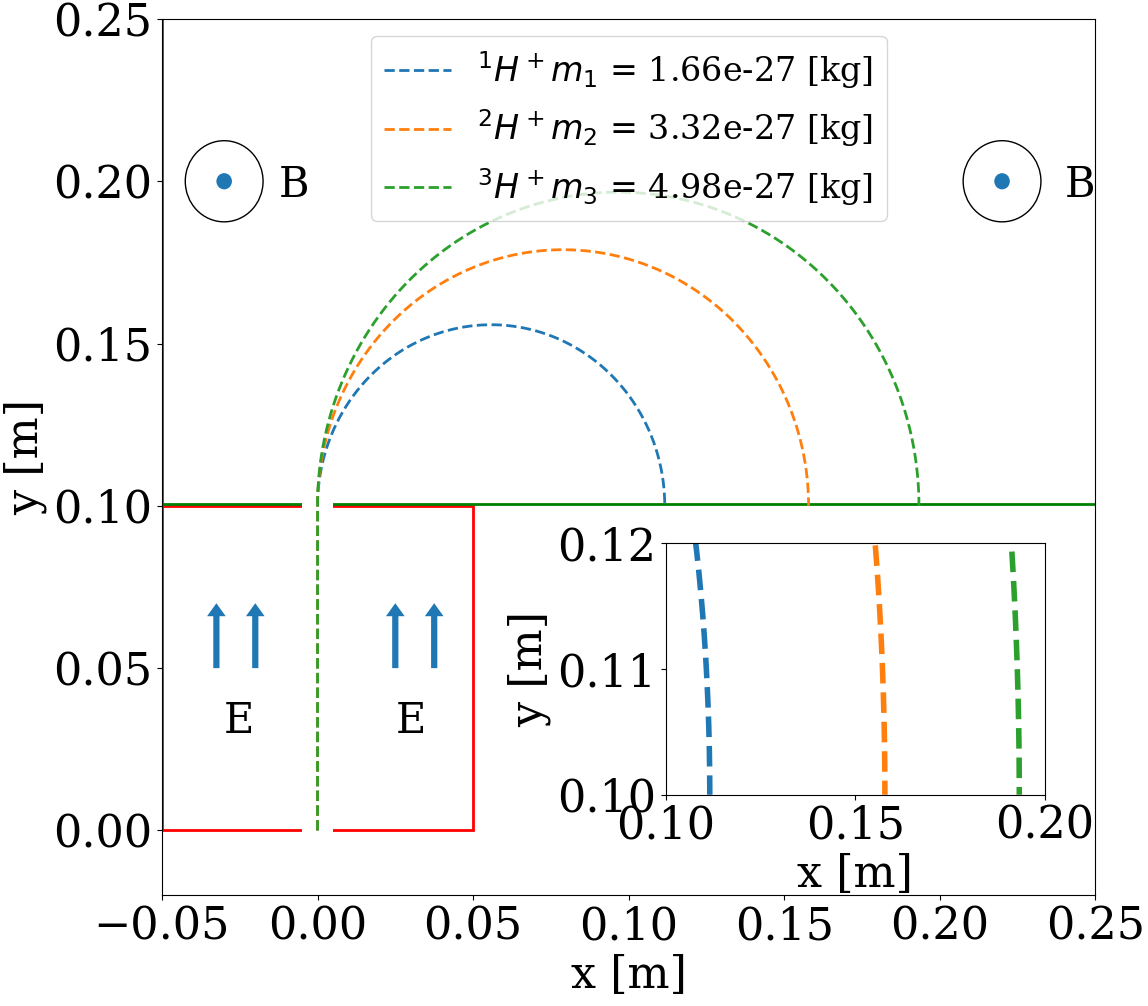
\includegraphics[width=\linewidth]{espectrometro_simulacion}
    \caption{Gráfica de simulación de espectrómetro de masa para los iones de hidrógeno $^1H^+$, $^2H^+$ y $^3H+$. El detalle muestra los puntos de impacto $x^s_1 = 1.11\cdot 10^{-1}~[m]$, $x^s_2 = 1.58\cdot 10^{-1}~[m]$, $x^s_3 = 1.93\cdot 10^{-1}~[m]$.}
    \label{fig:espectrometro_simulacion}
\end{figure}

\newpage

\section{Selector de Velocidades}
\label{sec:selector}

En el segundo apartado de la práctica estudiaremos el movimiento de uno de los iones ya mencionados en la sección anterior pero esta vez en el seno de otro instrumento: el selector de velocidades. En este caso, los iones procedentes de una fuente entran con una velocidad inicial al selector, dentro del cual existe tanto un campo eléctrico (perpendicular a la dirección de entrada) y un campo magnético (perpendicular tanto al campo eléctrico como a la dirección de entrada). Según el valor de los campos y la energía cinética del ion, la partícula en el interior se desviará en mayor o menor medida o bien no se desviará y realizará un movimiento rectilíneo consiguiendo salir del selector por una pequeña apertura en el extremo opuesto. De esta forma, eligiendo los valores adecuados para los campos se puede seleccionar aquellas partículas con una velocidad determinada. La Figura \ref{fig:selector} muestra un equema de dicho instrumento.

\begin{figure}[!htb]
    \includegraphics[width=\linewidth]{example-image-b}
    \caption{Representación esquemática del selector de velocidades de longitud $L$ con un campo eléctrico $E$ y magnético $B$ y una separación entre placas $2H$.}
    \label{fig:selector}
\end{figure}

Para resolver este problema fijaremos un campo eléctrico y variaremos el campo magnético hasta conseguir de forma experimental que la partícula salga por la rendija. Para que esto ocurra, la fuerza magnética debe compensar la fuerza eléctrica hasta cierto punto para que la partícula no sufra una desviación que le impida salir por la rendija. Para el cálculo tanto analítico como simulado emplearemos los siguientes datos de entrada:

\begin{itemize}
    \item La carga de uno de los iones anteriores $q = 1.6\cdot10^{-19}~[C]$ y su masa $m_1 = 1.66\cdot10^{-27}~[kg]$ para $^1H^+$.
    \item La energía cinética del ion al entrar en el selector $E_c = 30 [eV]$.
    \item La diferencia de potencial entre las placas $V = 25~[V]$.
    \item La distancia entre las placas horizonales $2H = 4\cdot 10^{-1}~[m]$.
    \item La longitud del selector $L = 2~[m]$.
    \item La apertura final del detector $2dy$ siendo $dy = 5\cdot10^{-2}H~[m]$.
\end{itemize}

\subsection{Cálculos Analíticos}

Dado que la fuerza total que actúa sobre la partícula viene dada por la fuerza de Lorent

\begin{equation}
    F = q(E + v \times B)~[N],
\end{equation}

para conseguir que la partícula siga una trayectoria rectilínea y por lo tanto sea capaz de alcanzar la rendija es necesario que la fuerza ejercida por el campo eléctrico sea compensada por la fuerza realizada por el campo eléctrico

\begin{equation}
    F_e = F_m \Rightarrow qE = qvB,
\end{equation}

de lo cual deducimos que la velocidad del ión que será seleccionado (capaz de alcanzar la rendija sin desviarse significativamente) será

\begin{equation}
    v = \displaystyle\frac{E}{B}~[m\cdot s].
\end{equation}

Así pues, ajustando los valores de ambos campos podemos hacer que únicamente las partículas con una determinada velocidad de entrada $v$ sigan una trayectoria rectilínea. Aquellas con una velocidad menor se verán más influenciadas por la fuerza eléctrica y por lo tanto se desviarán hacia arriba mientras que aquellas con una velocidad mayor sufrirán una fuerza magnética más intensa y se desviarán hacia abajo. Si esta desviación es demasiado pronunciada, no conseguirán alcanzar la rendija.

Para el caso que nos ocupa, el ión $^1H^+$, sabemos que su masa es de $m = 1.66\cdot 10^{-27}~[kg]$ y su carga es $q = 1.6 \cdot 10^{-19}~[C]$. La energía cinética de dicha partícula la hemos fijado en $30~[eV]$ ($30\cdot 1.6\cdot 10^{-19}~[J]$) por lo que a partir de la misma podemos obtener su velocidad

\begin{equation}
    E_c = \displaystyle\frac{1}{2}mv^2 \Rightarrow v = \sqrt{\displaystyle\frac{2E_c}{m}} = 7.6\cdot 10^4~[m\cdot s^{-1}]~.
\end{equation}

Dado que hemos fijado una diferencia de potencial de $V = 25~[V]$ y una distancia entre las placas horizontales de $2H = 4\cdot 10^{-1}~[m]$, podemos calcular el campo eléctrico $E$ como

\begin{equation}
    V = Ed \Rightarrow E = \displaystyle\frac{V}{2H} = \displaystyle\frac{25}{2\cdot 4\cdot 10^{-1}} = 6.25~[V\cdot m^{-1}]~.
\end{equation}

Por lo tanto, el campo magnético que necesitaremos para compensar la fuerza eléctrica con el objetivo de seleccionar la velocidad $v$ dada es

\begin{equation}
    v = \displaystyle\frac{E}{B} \Rightarrow B = \displaystyle\frac{E}{v} = \displaystyle\frac{6.25}{7.6\cdot 10^4} = 8.21 \cdot 10^{-4}~[T]~.
\end{equation}

\subsection{Simulación}

Durante la simulación, hemos variado el campo magnético sin conocer el valor analítico hasta conseguir que el ión atraviese la rendija utilizando los valores de energía cinética y de campo eléctrico (diferencia de potencial y distancia entre las placas) seleccionados anteriormente (ver Código \ref{listing:datos_selector}). Finalmente, llegamos a la conclusión de que el valor analítico $B = 8.21\cdot 10^{-4}~[T]$ permite al ión alcanzar la rendija sin desviarse tal y como se muestra en la Figura \ref{fig:selector_simulacion}.

\newpage

\begin{code}
    \begin{minted}{python}
# Datos de entrada
# El programa calcula la trayectoria en un
# selector de velocidad de un ion con una
# dada velocidad, y la del mismo ion pero
# con una velocidad 10 % mayor y 10% menor

# Masa del ion
m=1.0e-3 / 6.022e23  
#Carga del ion
q=1.6e-19   
# 2*H es la distancia entre las placas horizontales
H=0.2
# Diferencia de potencial entre ambas placas  
dV=25     
E=dV/2./H   # Campo eléctrico uniforme
# Campo magnético
B=8.21e-4  
# Distancia horizontal del selector
L=2.0  
# Energía cinética del ion que entra
Ec=30*1.6e-19  
#Velocidad del ion que entra al selector
vx0=np.sqrt(2*Ec/m)  
# 2*dy es el tamaño de la apertura
dy=0.05 * H 

#tiempo final de simulacion
tf=10.0           
    \end{minted}
    \caption{Datos de simulación de selector de velocidad.}
    \label{listing:datos_selector}
\end{code}

\begin{figure}[!htb]
    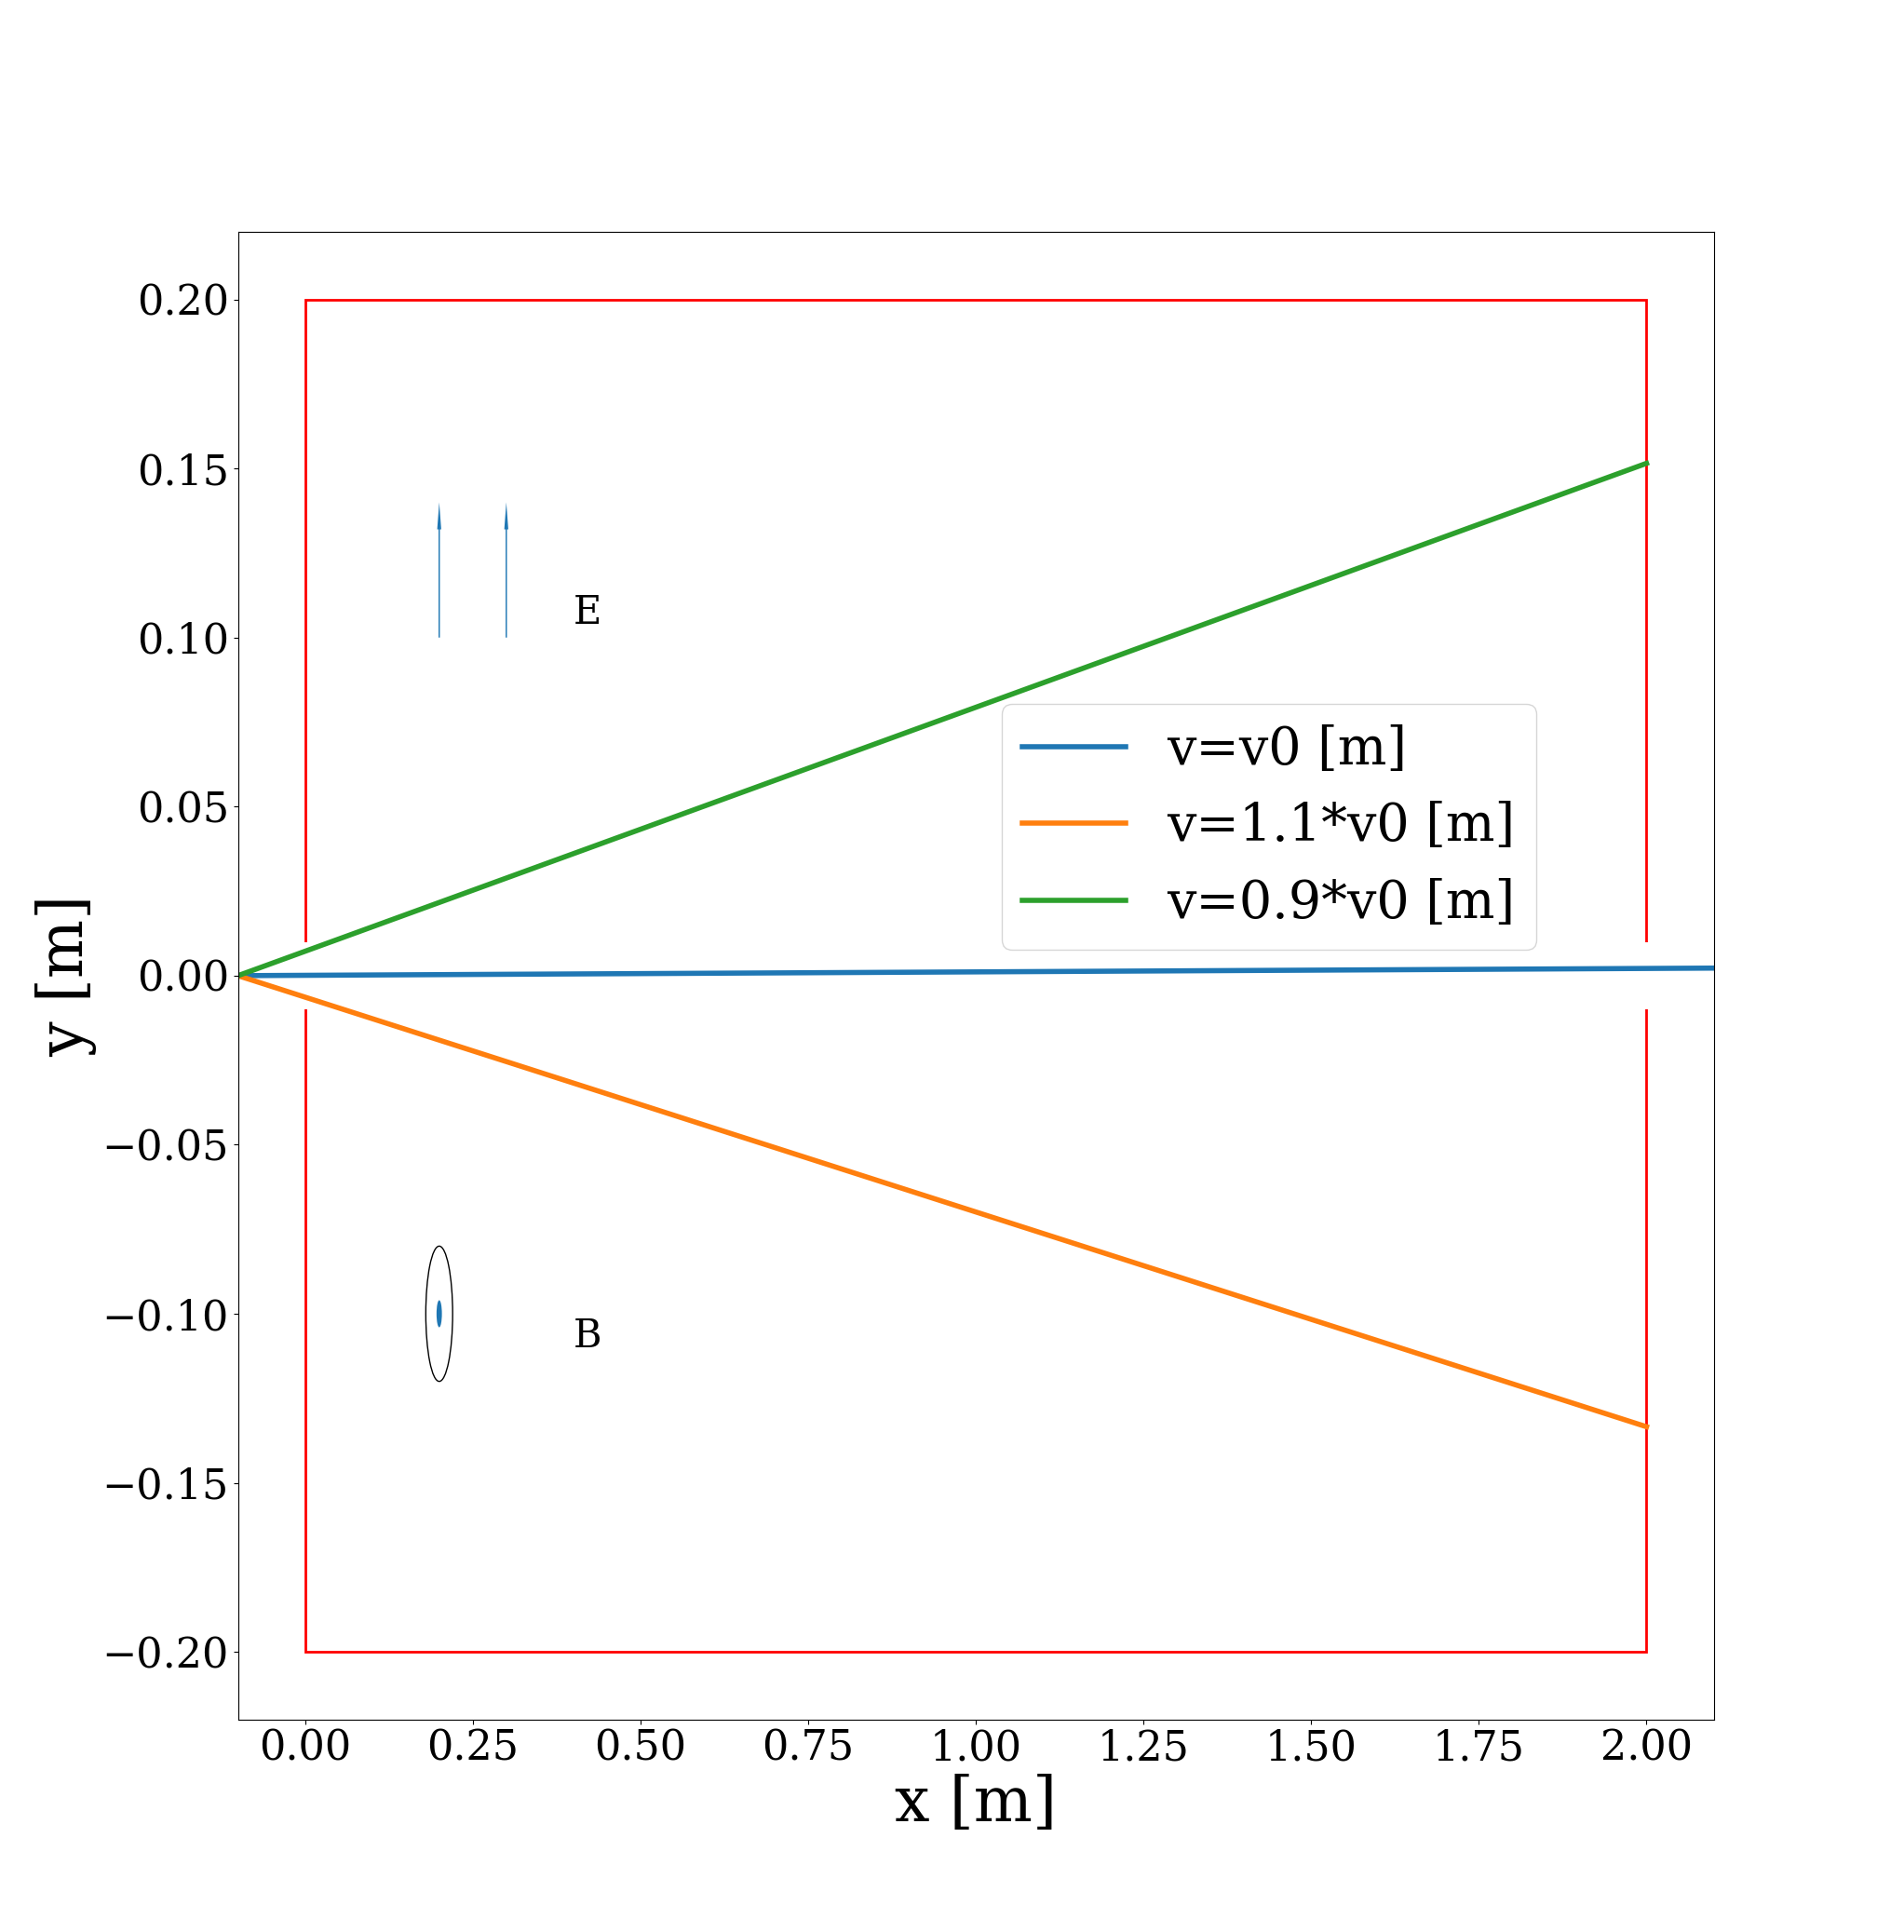
\includegraphics[width=\linewidth]{selector_simulacion}
    \caption{Gráfica de simulación de selector de velocidad con $v_0 = 7.6\cdot 10^4~[m\cdot s^{-1}]$, $E = 6.25~[V\cdot m^{-1}]$ y $B = 8.21\cdot 10^{-4}~[T]$ tal y como calculamos de forma analítica. Como podemos observar, el ión es capaz de alcanzar la rendija. La simulación también muestra el resultado de utilizar un $90\%$ de la velocidad inicial (el campo eléctrico desvía el ión hacia arriba) y utilizar un $110\%$ de la misma (el campo magnético desvía el ión hacia abajo).}
    \label{fig:selector_simulacion}
\end{figure}

\clearpage

\section{Ciclotrón}
\label{sec:ciclotron}

En esta sección de la práctica trataremos el movimiento de protones en un ciclotrón (ver Figura \ref{fig:ciclotron}), un instrumento en el que una partícula cargada es acelerada inicialmente desde el reposo mediante la acción de un campo eléctrico existente en la región de separación entre los dos semicírculos denominados $Ds$ del ciclotrón. En los semicírculos existe un campo magnético que les produce un movimiento circular cuyo radio depende de la velocidad con la que provengan de la región del campo eléctrico que los ha acelerado. Ese movimiento circular les hace volver a la región del campo eléctrico que varía de manera periódica para acelerar los protones hacia la $D$ opuesta. Con el tiempo y tras varios pasos por la región del campo eléctrico y por las $D$ las partículas son capaces de ganar grandes cantidades de energía y alcanzar velocidades tremendamente elevadas.

\begin{figure}[!htb]
    \includegraphics[width=\linewidth]{example-image-c}
    \caption{Representación esquemática del ciclotrón con un campo magnético $B$, radio $R$ y distancia $d$.}
    \label{fig:ciclotron}
\end{figure}

\subsection{Cálculos Analíticos}



\subsection{Simulación}

\clearpage

\section{Frecuencia de Ciclotrón Relativista}
\label{sec:frecuencia}

Para resolver este problema elegiremos una partícula, en nuestro caso el protón, y escogeremos para la misma una serie de valores para la velocidad (entre $1\cdot 10^2~[m\cdot s^{-1}]$ y $1\cdot 10^84[m\cdot s^{-1}]$) así como el campo magnético fijo del ciclotrón. De esta forma, los datos de entrada serán los siguientes:

\begin{itemize}
    \item Masa $m = 1.67\cdot 10^{-27}~[kg]$ y carga $q = 1.6\cdot 10^{-19}~[C]$ de la partícula (protón).
    \item Velocidades de la partícula $1\cdot 10^2~[m\cdot s^{-1}]$, $0.2\cdot 10^8~[m\cdot s^{-1}]$, $0.6\cdot 10^8~[m\cdot s^{-1}]$, $0.8\cdot 10^8~[m\cdot s^{-1}]$ y $1\cdot 10^8~[m\cdot s^{-1}]$.
    \item Campo magnético $B = 1~[T]$.
\end{itemize}

\subsection{Cálculos Analíticos}

En primer lugar, trataremos de obtener el radio de la curva que describe el protón en el ciclotrón una vez abandona el campo eléctrico y se ve sometido a una aceleración causada por el campo magnético en cada una de las Ds. Dicho campo magnético provoca la aparición de una fuerza magnética sobre la partícula ya que esta se desplaza con velocidad perpendicular al mismo. Esta fuerza hace que describa un movimiento circular cuyo radio podemos determinar como en el caso del espectrómetro de masas para velocidades no relativistas

\begin{equation}
F_m = ma_c \Rightarrow qvB = m \displaystyle\frac{v^2}{r} \Rightarrow r = \displaystyle\frac{mv}{qB}~[m]~.
\end{equation}

Para el caso de velocidades relativistas, la fórmula es idéntica pero reemplazando la masa invariante $m$ por la masa relativista $m\gamma$ siendo la constante

\begin{equation}
\gamma = \displaystyle\frac{1}{\sqrt{(1-\displaystyle\frac{v^2}{c^2})}},
\end{equation}

por lo tanto el radio de curvatura en el caso relativista es

\begin{equation}
r_\gamma = \displaystyle\frac{m\gamma v}{qB} = \displaystyle\frac{mv}{qB\sqrt{(1-\displaystyle\frac{v^2}{c^2})}}~[m]~.
\end{equation}

El período se puede calcular para el caso no relativista como

\begin{equation}
T = \displaystyle\frac{2\pi r}{v} = \displaystyle\frac{2\pi mv}{qBv} = \displaystyle\frac{2\pi m}{qB}~[s]~.
\end{equation}

Como podemos comprobar, no depende de la velocidad. El análogo relativista sí que depende de la misma puesto que la masa lo hace

\begin{equation}
T_\gamma = \displaystyle\frac{2\pi m\gamma}{qB} = \displaystyle\frac{2\pi m}{qB\sqrt{(1-\displaystyle\frac{v^2}{c^2})}} ~[s]~.
\end{equation}

La frecuencia en ambos casos es la inversa del período

\begin{equation}
    f = \displaystyle\frac{1}{T} = \displaystyle\frac{qB}{2\pi m}~[Hz]~.
\end{equation}

\begin{equation}
    f_\gamma = \displaystyle\frac{1}{T_\gamma} = \displaystyle\frac{qB\sqrt{(1-\displaystyle\frac{v^2}{c^2})}}{2\pi m}~[Hz]~.
\end{equation}

\subsubsection{$v_1 = 1.0\cdot 10^2~[m\cdot s^{-1}]$}

Para la primera velocidad seleccionada estamos ante un caso no relativista. Dada la escasa velocidad, la constante $\gamma$ se aproxima a $1.00$ por lo que la masa relativista es prácticamente igual a la masa invariante

\begin{equation}
\gamma_1 = \displaystyle\frac{1}{\sqrt{(1-\displaystyle\frac{v_1^2}{c^2})}} = \displaystyle\frac{1}{\sqrt{(1-\displaystyle\frac{(1.0\cdot 10^2)^2}{(3\cdot 10^8)^2})}} \simeq 1.00
\end{equation}

Su radio de curvatura es por lo tanto

\begin{equation}
r_1 = \displaystyle\frac{mv_1}{qB} = \displaystyle\frac{1.67\cdot 10^{-27}\cdot 1.0\cdot 10^2}{1.6\cdot 10^{-19}\cdot 1} = 1.04\cdot 10^{-6}~[m]~.
\end{equation}

Su período es

\begin{equation}
T_1 = \displaystyle\frac{2\pi m}{qB} = \displaystyle\frac{2\pi \cdot 1.67\cdot 10^{-27}}{1.6\cdot 10^{-19}\cdot 1.0} = 6.56\cdot 10^{-8}~[s]~,
\end{equation}

y por lo tanto la frecuencia es

\begin{equation}
f_1 = \displaystyle\frac{1}{T_1} = \displaystyle\frac{1}{6.56\cdot 10^{-8}} = 1.52\cdot 10^7~[Hz]~.
\end{equation}

\subsubsection{$v_2 = 0.2\cdot 10^8~[m\cdot s^{-1}]$}

Para la segunda velocidad seleccionada nos encontramos ante un caso relativista. La velocidad cercana a la velocidad de la luz hace que la constante $\gamma$ sea superior a $1.00$ por lo que la masa relativista es mayor que la masa invariante 

\begin{equation}
\gamma_2 = \displaystyle\frac{1}{\sqrt{(1-\displaystyle\frac{v_2^2}{c^2})}} = \displaystyle\frac{1}{\sqrt{(1-\displaystyle\frac{(0.2\cdot 10^8)^2}{(3\cdot 10^8)^2})}} \simeq 1.002
\end{equation}

Su radio de curvatura es por lo tanto

\begin{equation}
r_2 = \displaystyle\frac{m\gamma_2v_2}{qB} = \displaystyle\frac{1.67\cdot 10^{-27}\cdot 1.002 \cdot 0.2\cdot 10^8}{1.6\cdot 10^{-19}\cdot 1} = 2.09\cdot 10^{-1}~[m]~.
\end{equation}

\subsubsection{$v_3 = 0.6\cdot 10^8~[m\cdot s^{-1}]$}

Para la tercera velocidad, la constante $\gamma$ es todavía mayor

\begin{equation}
\gamma_3 = \displaystyle\frac{1}{\sqrt{(1-\displaystyle\frac{v_3^2}{c^2})}} = \displaystyle\frac{1}{\sqrt{(1-\displaystyle\frac{(0.6\cdot 10^8)^2}{(3\cdot 10^8)^2})}} \simeq 1.020
\end{equation}

Su radio de curvatura es por lo tanto

\begin{equation}
r_3 = \displaystyle\frac{m\gamma_3v_3}{qB} = \displaystyle\frac{1.67\cdot 10^{-27}\cdot 1.020 \cdot 0.6\cdot 10^8}{1.6\cdot 10^{-19}\cdot 1} = 6.39\cdot 10^{-1}~[m]~.
\end{equation}

\subsubsection{$v_4 = 0.8\cdot 10^8~[m\cdot s^{-1}]$}

En el caso de la cuarta velocidad, $\gamma$ continúa creciendo

\begin{equation}
\gamma_4 = \displaystyle\frac{1}{\sqrt{(1-\displaystyle\frac{v_4^2}{c^2})}} = \displaystyle\frac{1}{\sqrt{(1-\displaystyle\frac{(0.8\cdot 10^8)^2}{(3\cdot 10^8)^2})}} \simeq 1.037
\end{equation}

Su radio de curvatura es por lo tanto

\begin{equation}
r_4 = \displaystyle\frac{m\gamma_4v_4}{qB} = \displaystyle\frac{1.67\cdot 10^{-27}\cdot 1.037 \cdot 0.8\cdot 10^8}{1.6\cdot 10^{-19}\cdot 1} = 8.66\cdot 10^{-1}~[m]~.
\end{equation}

\subsubsection{$v_5 = 1.0\cdot 10^8~[m\cdot s^{-1}]$}

La quinta velocidad posee la constante $\gamma$ más elevada

\begin{equation}
\gamma_5 = \displaystyle\frac{1}{\sqrt{(1-\displaystyle\frac{v_5^2}{c^2})}} = \displaystyle\frac{1}{\sqrt{(1-\displaystyle\frac{(1.0\cdot 10^8)^2}{(3\cdot 10^8)^2})}} \simeq 1.061
\end{equation}

Su radio de curvatura es por lo tanto

\begin{equation}
r_5 = \displaystyle\frac{m\gamma_5v_5}{qB} = \displaystyle\frac{1.67\cdot 10^{-27}\cdot 1.061 \cdot 1.0\cdot 10^8}{1.6\cdot 10^{-19}\cdot 1} = 1.11 ~[m]~.
\end{equation}

\subsection{Simulación}

\begin{figure}
    \centering
    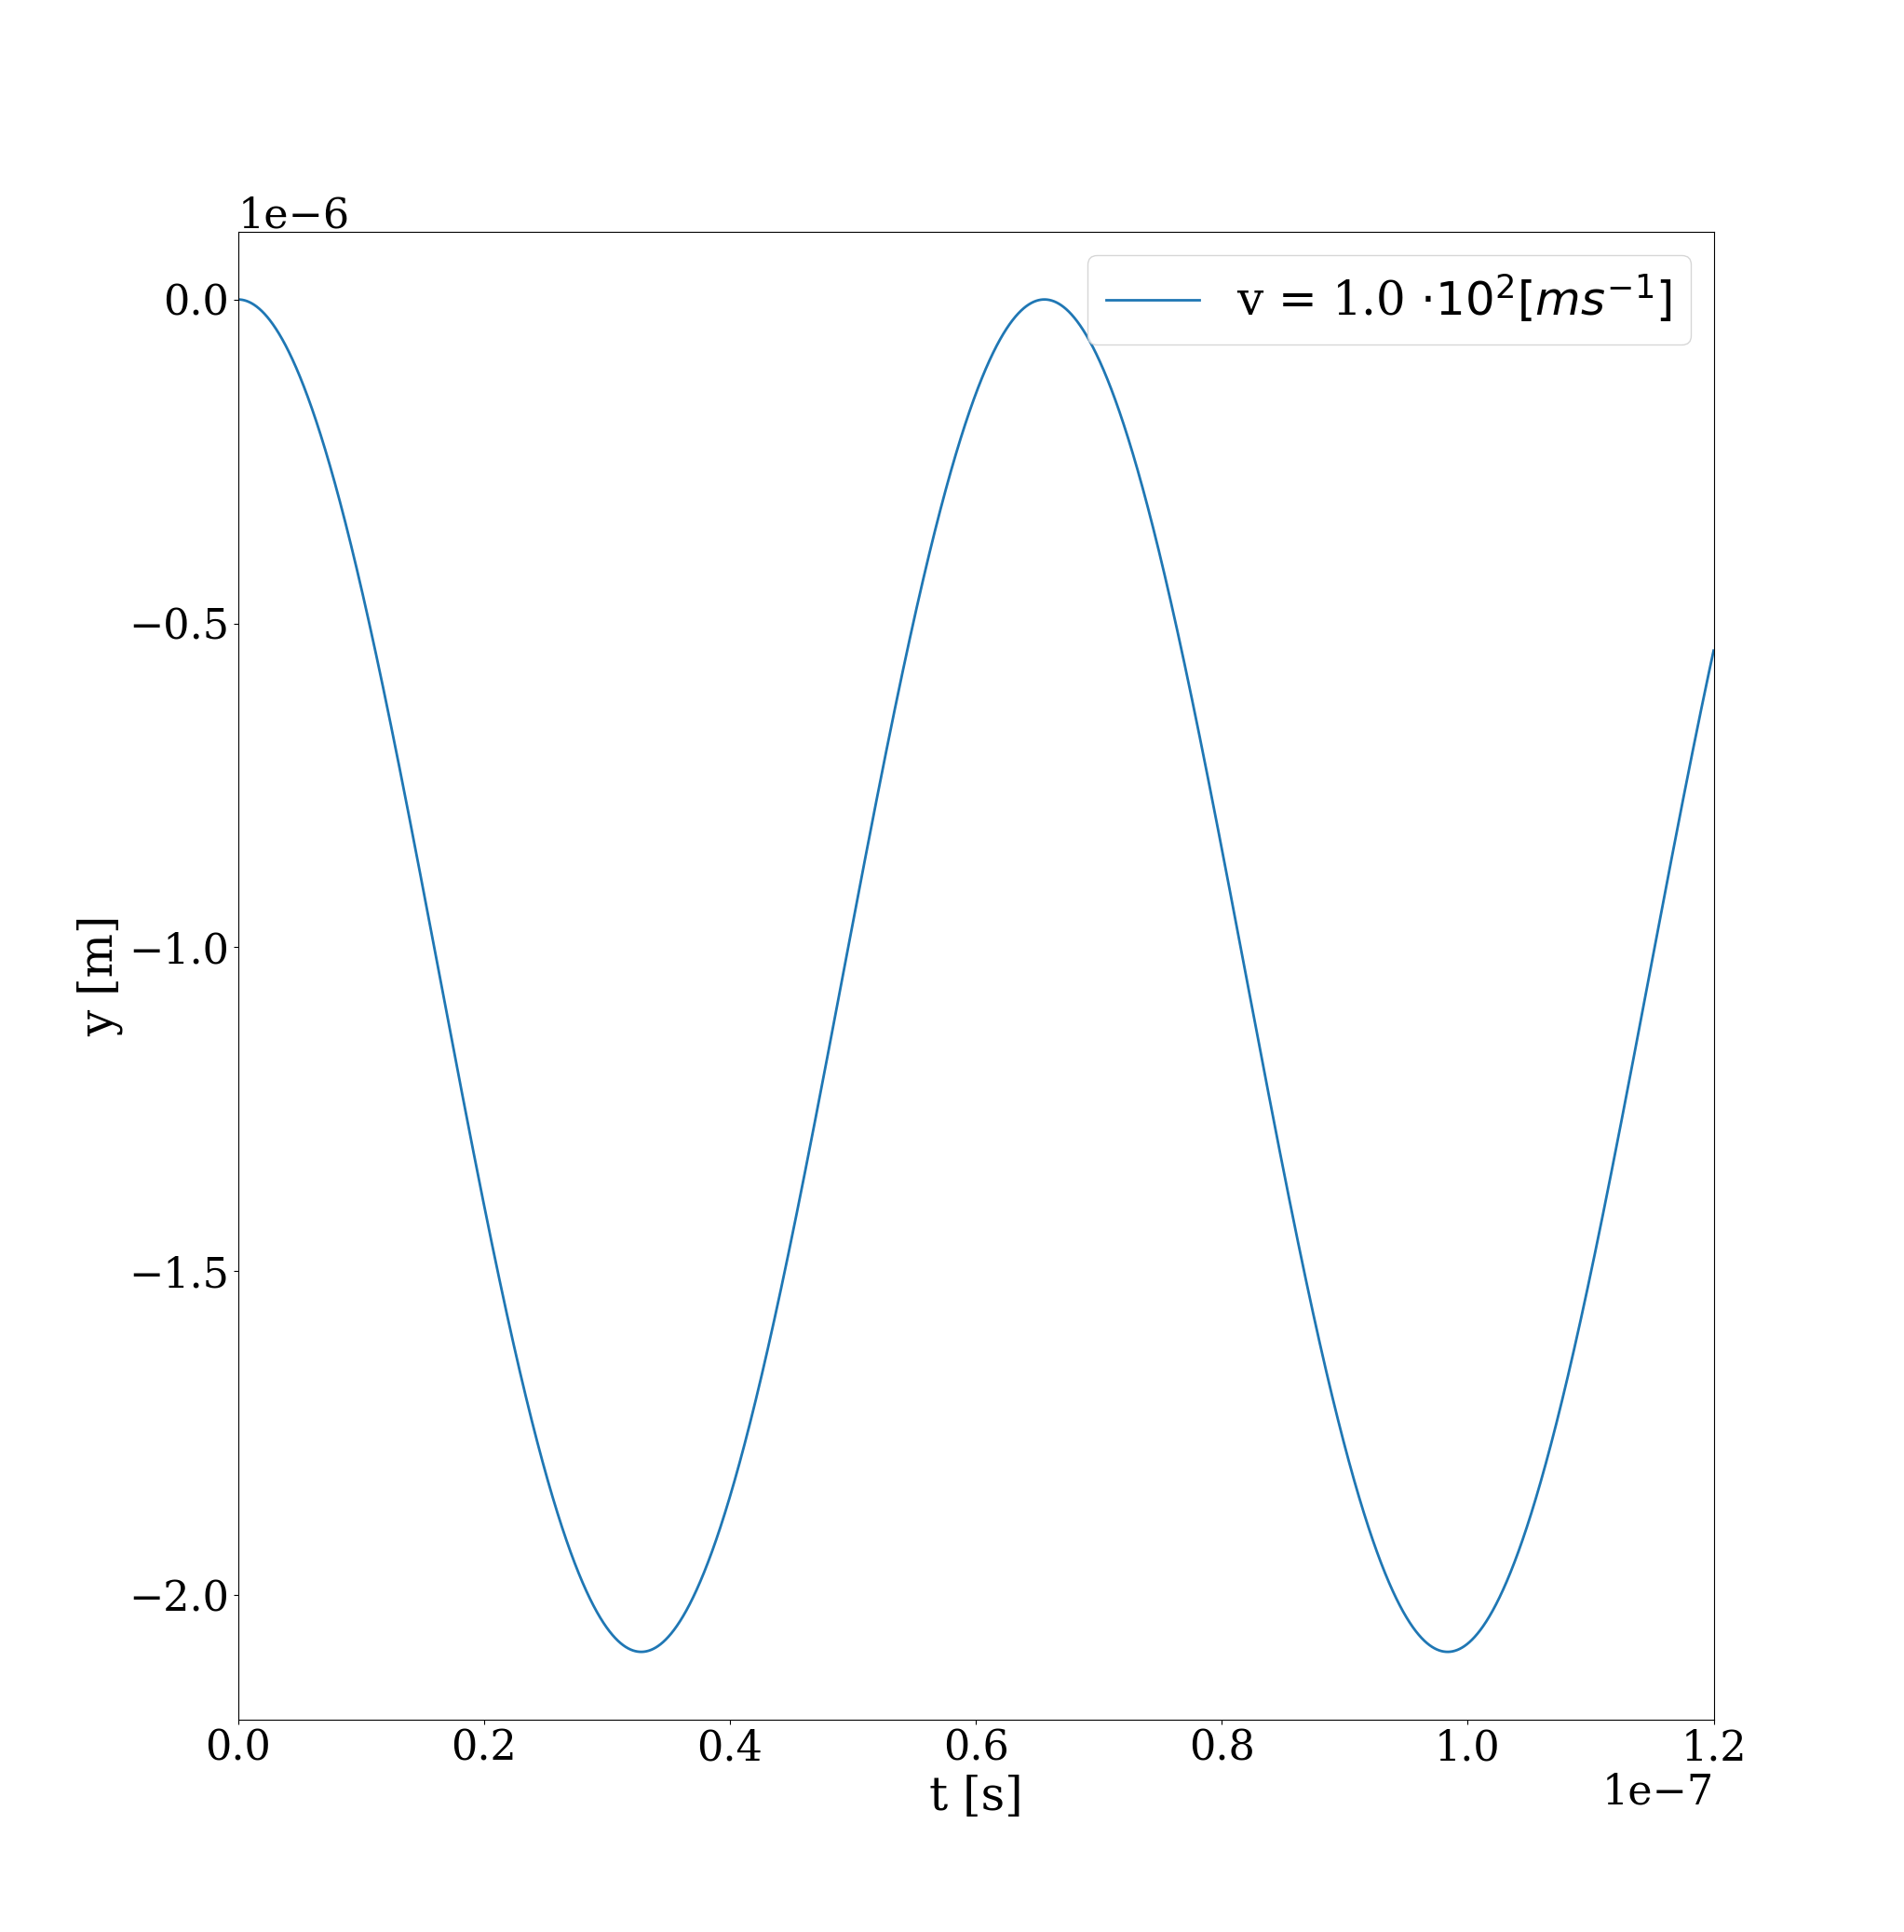
\includegraphics[width=\linewidth]{freq_rel_1.png}
\end{figure}

\begin{figure}
    \centering
    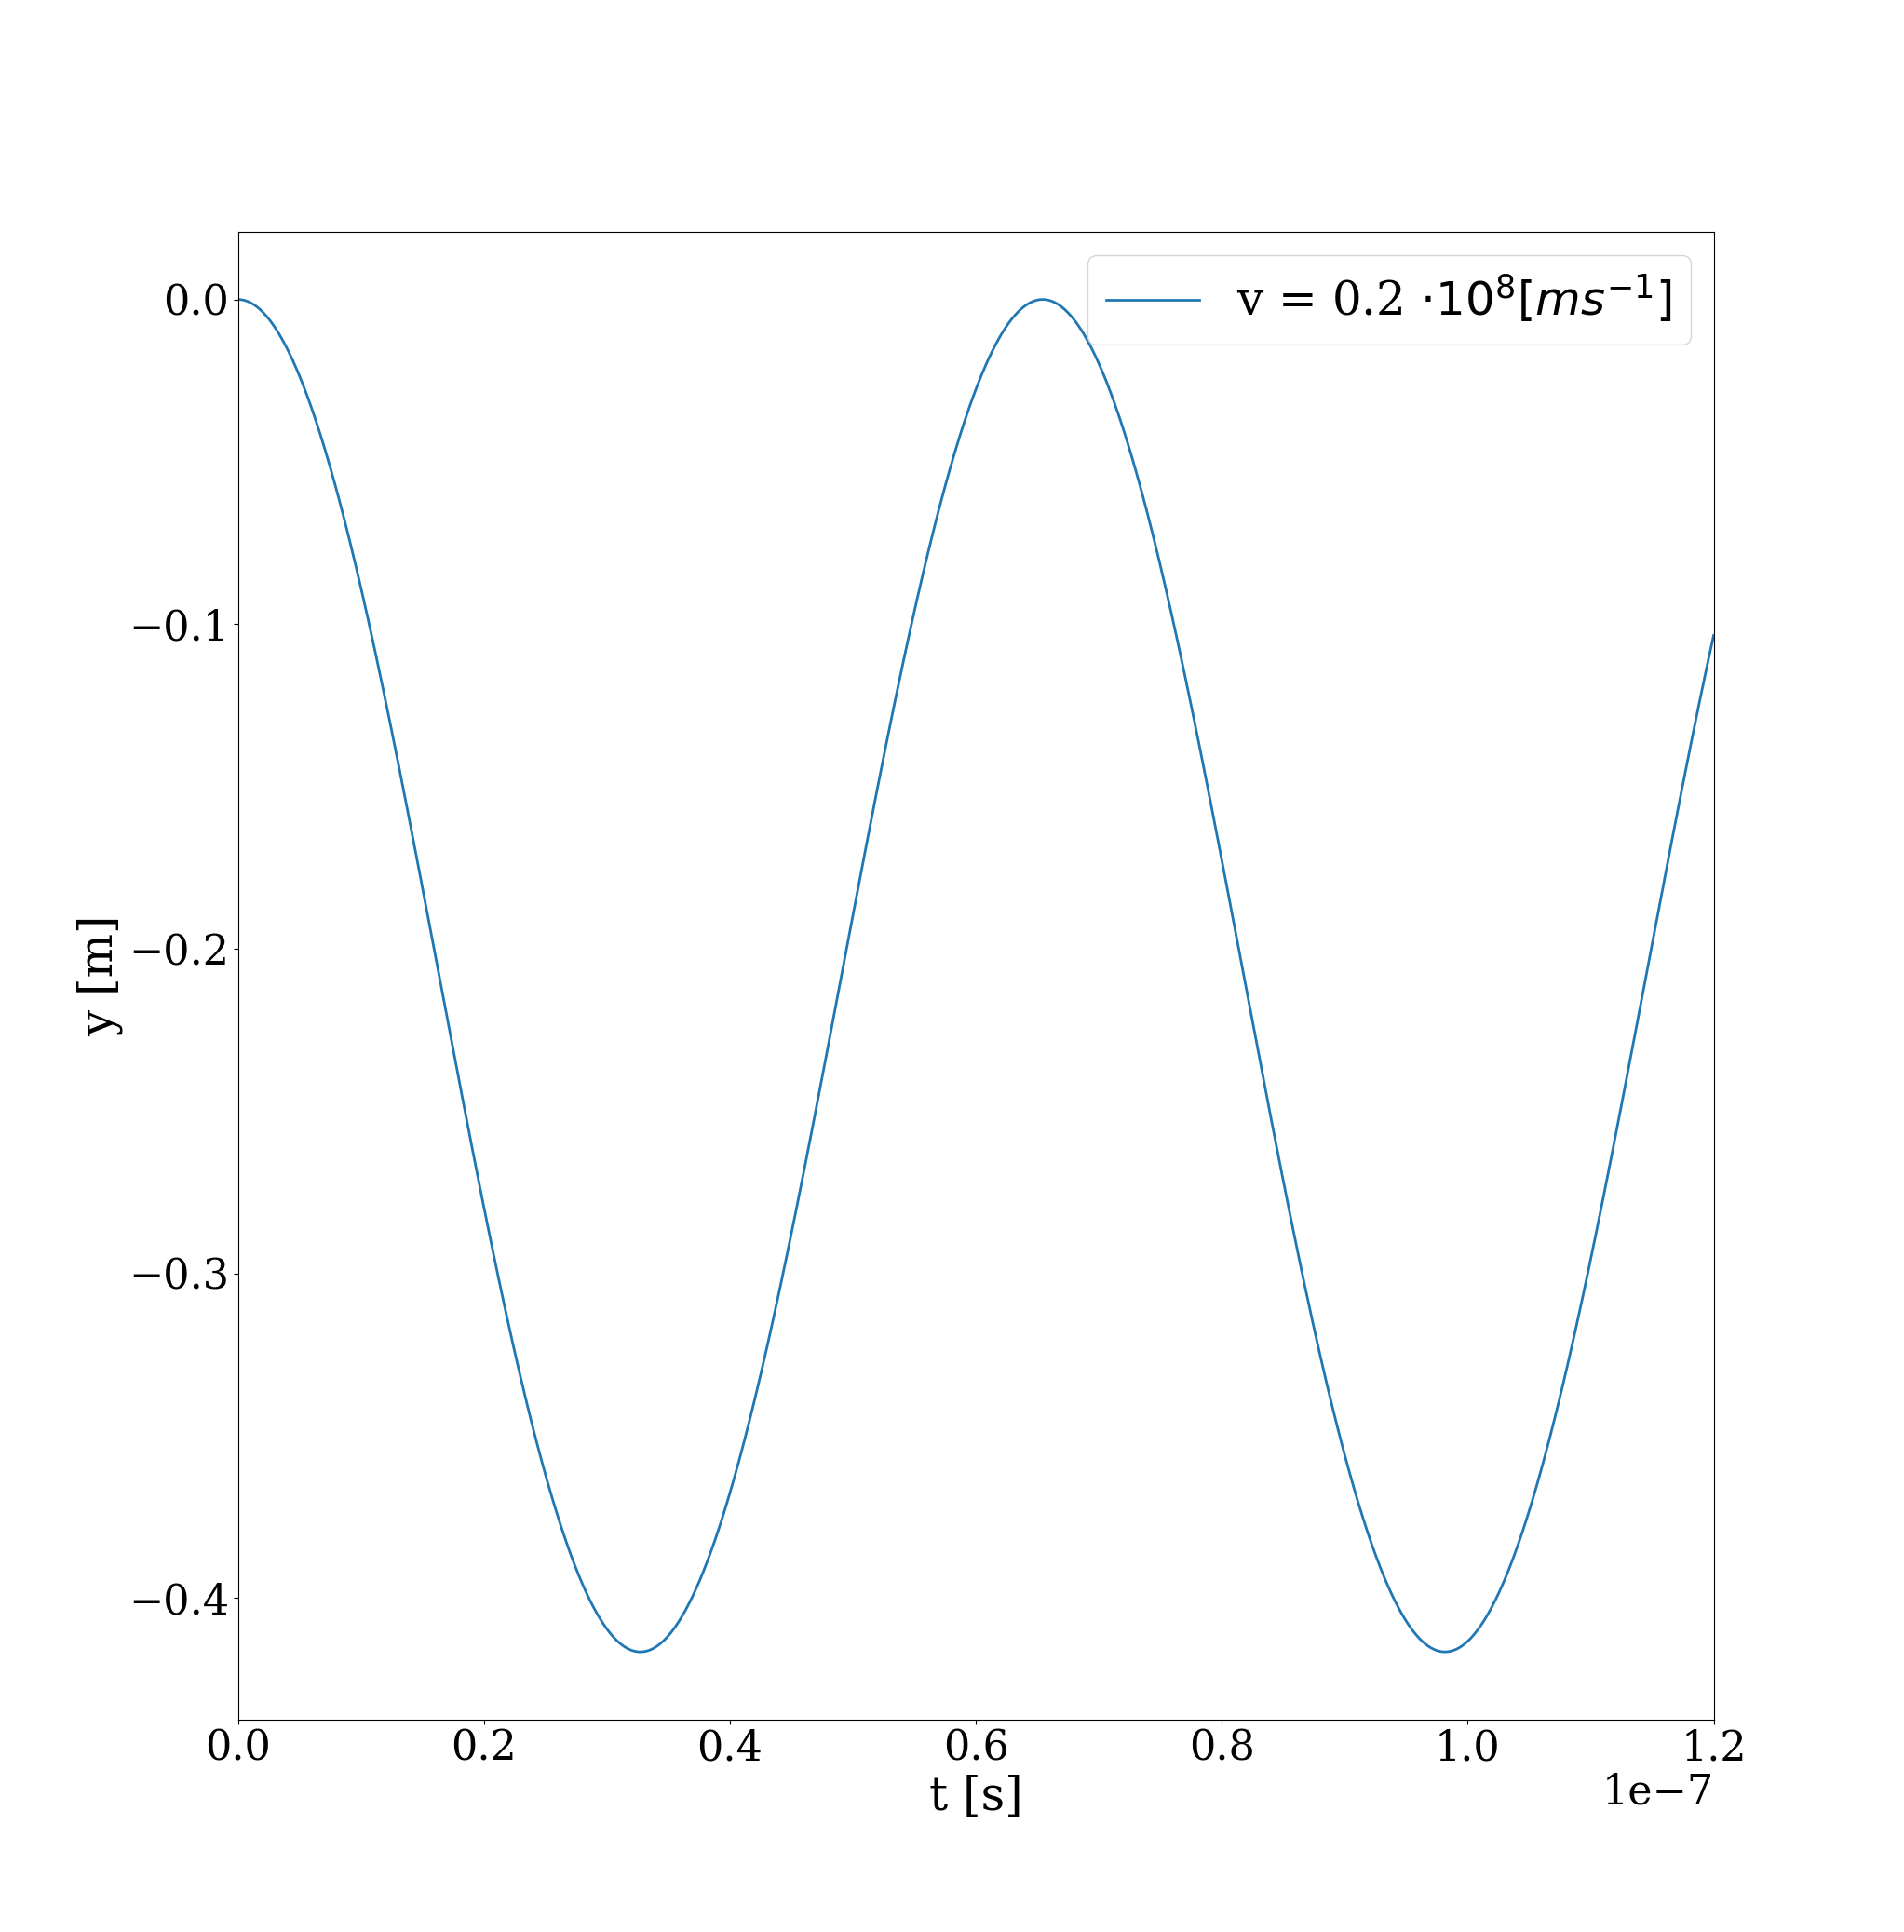
\includegraphics[width=\linewidth]{freq_rel_2.png}
\end{figure}

\begin{figure}
    \centering
    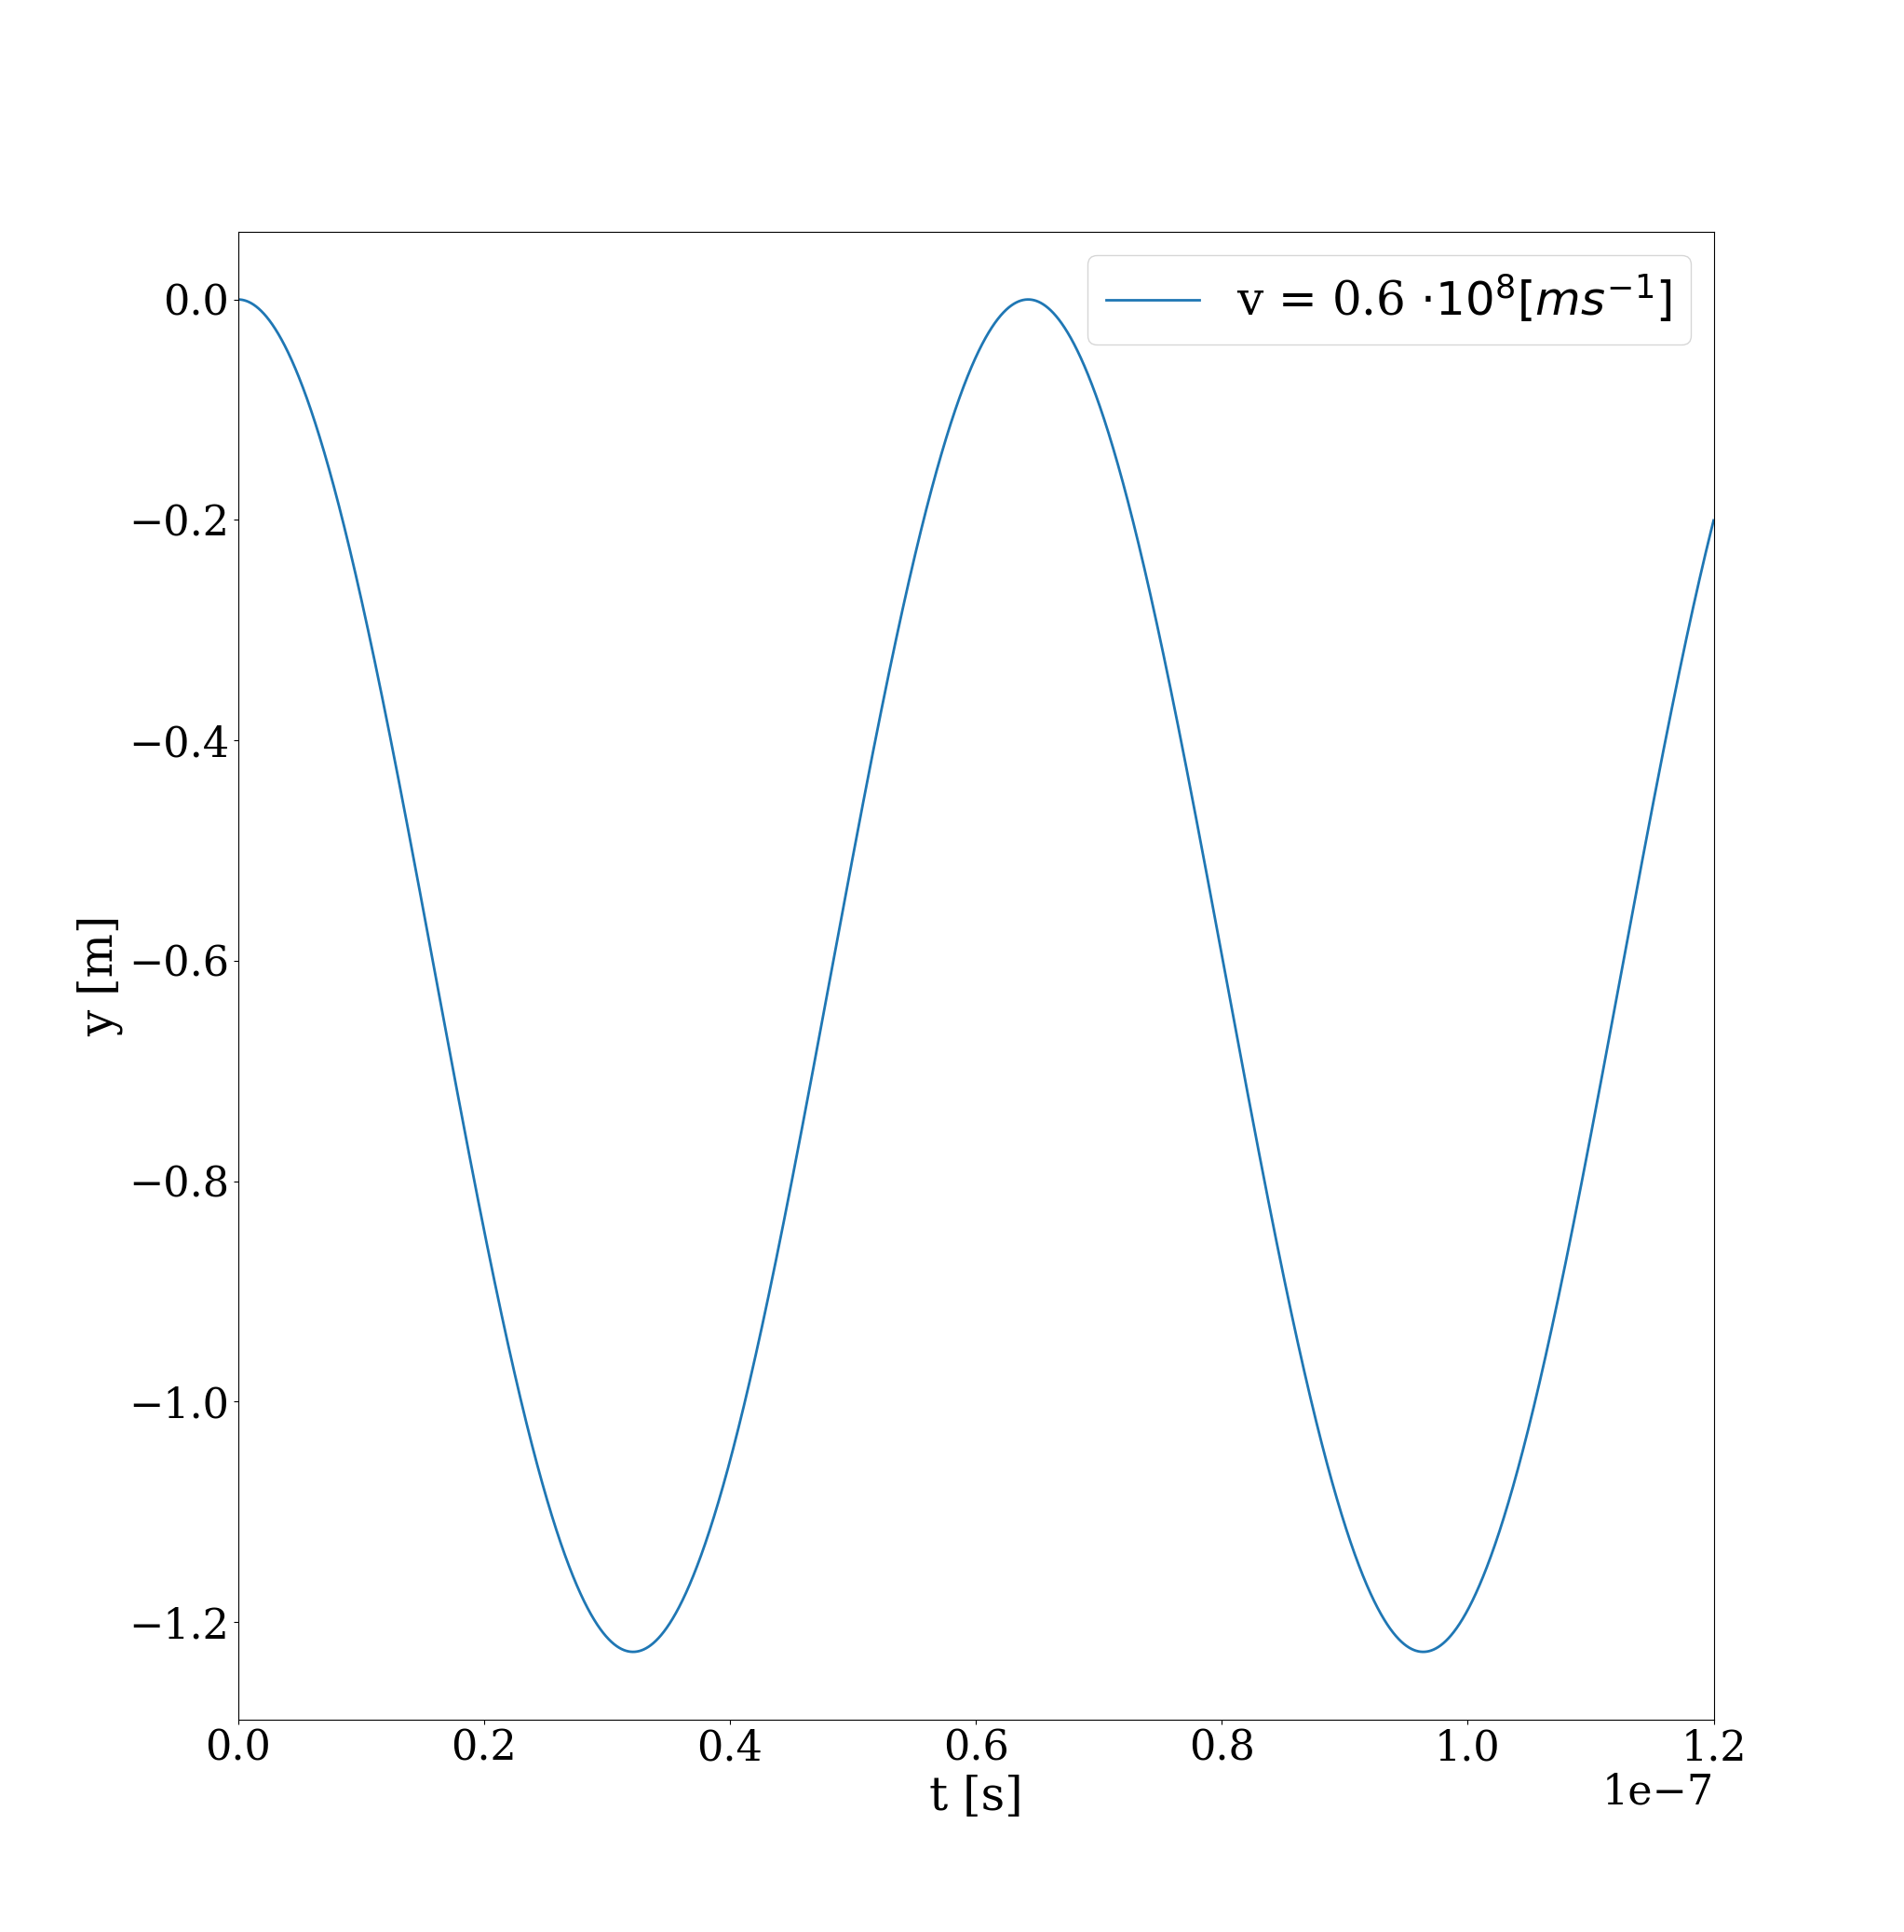
\includegraphics[width=\linewidth]{freq_rel_3.png}
\end{figure}

\begin{figure}
    \centering
    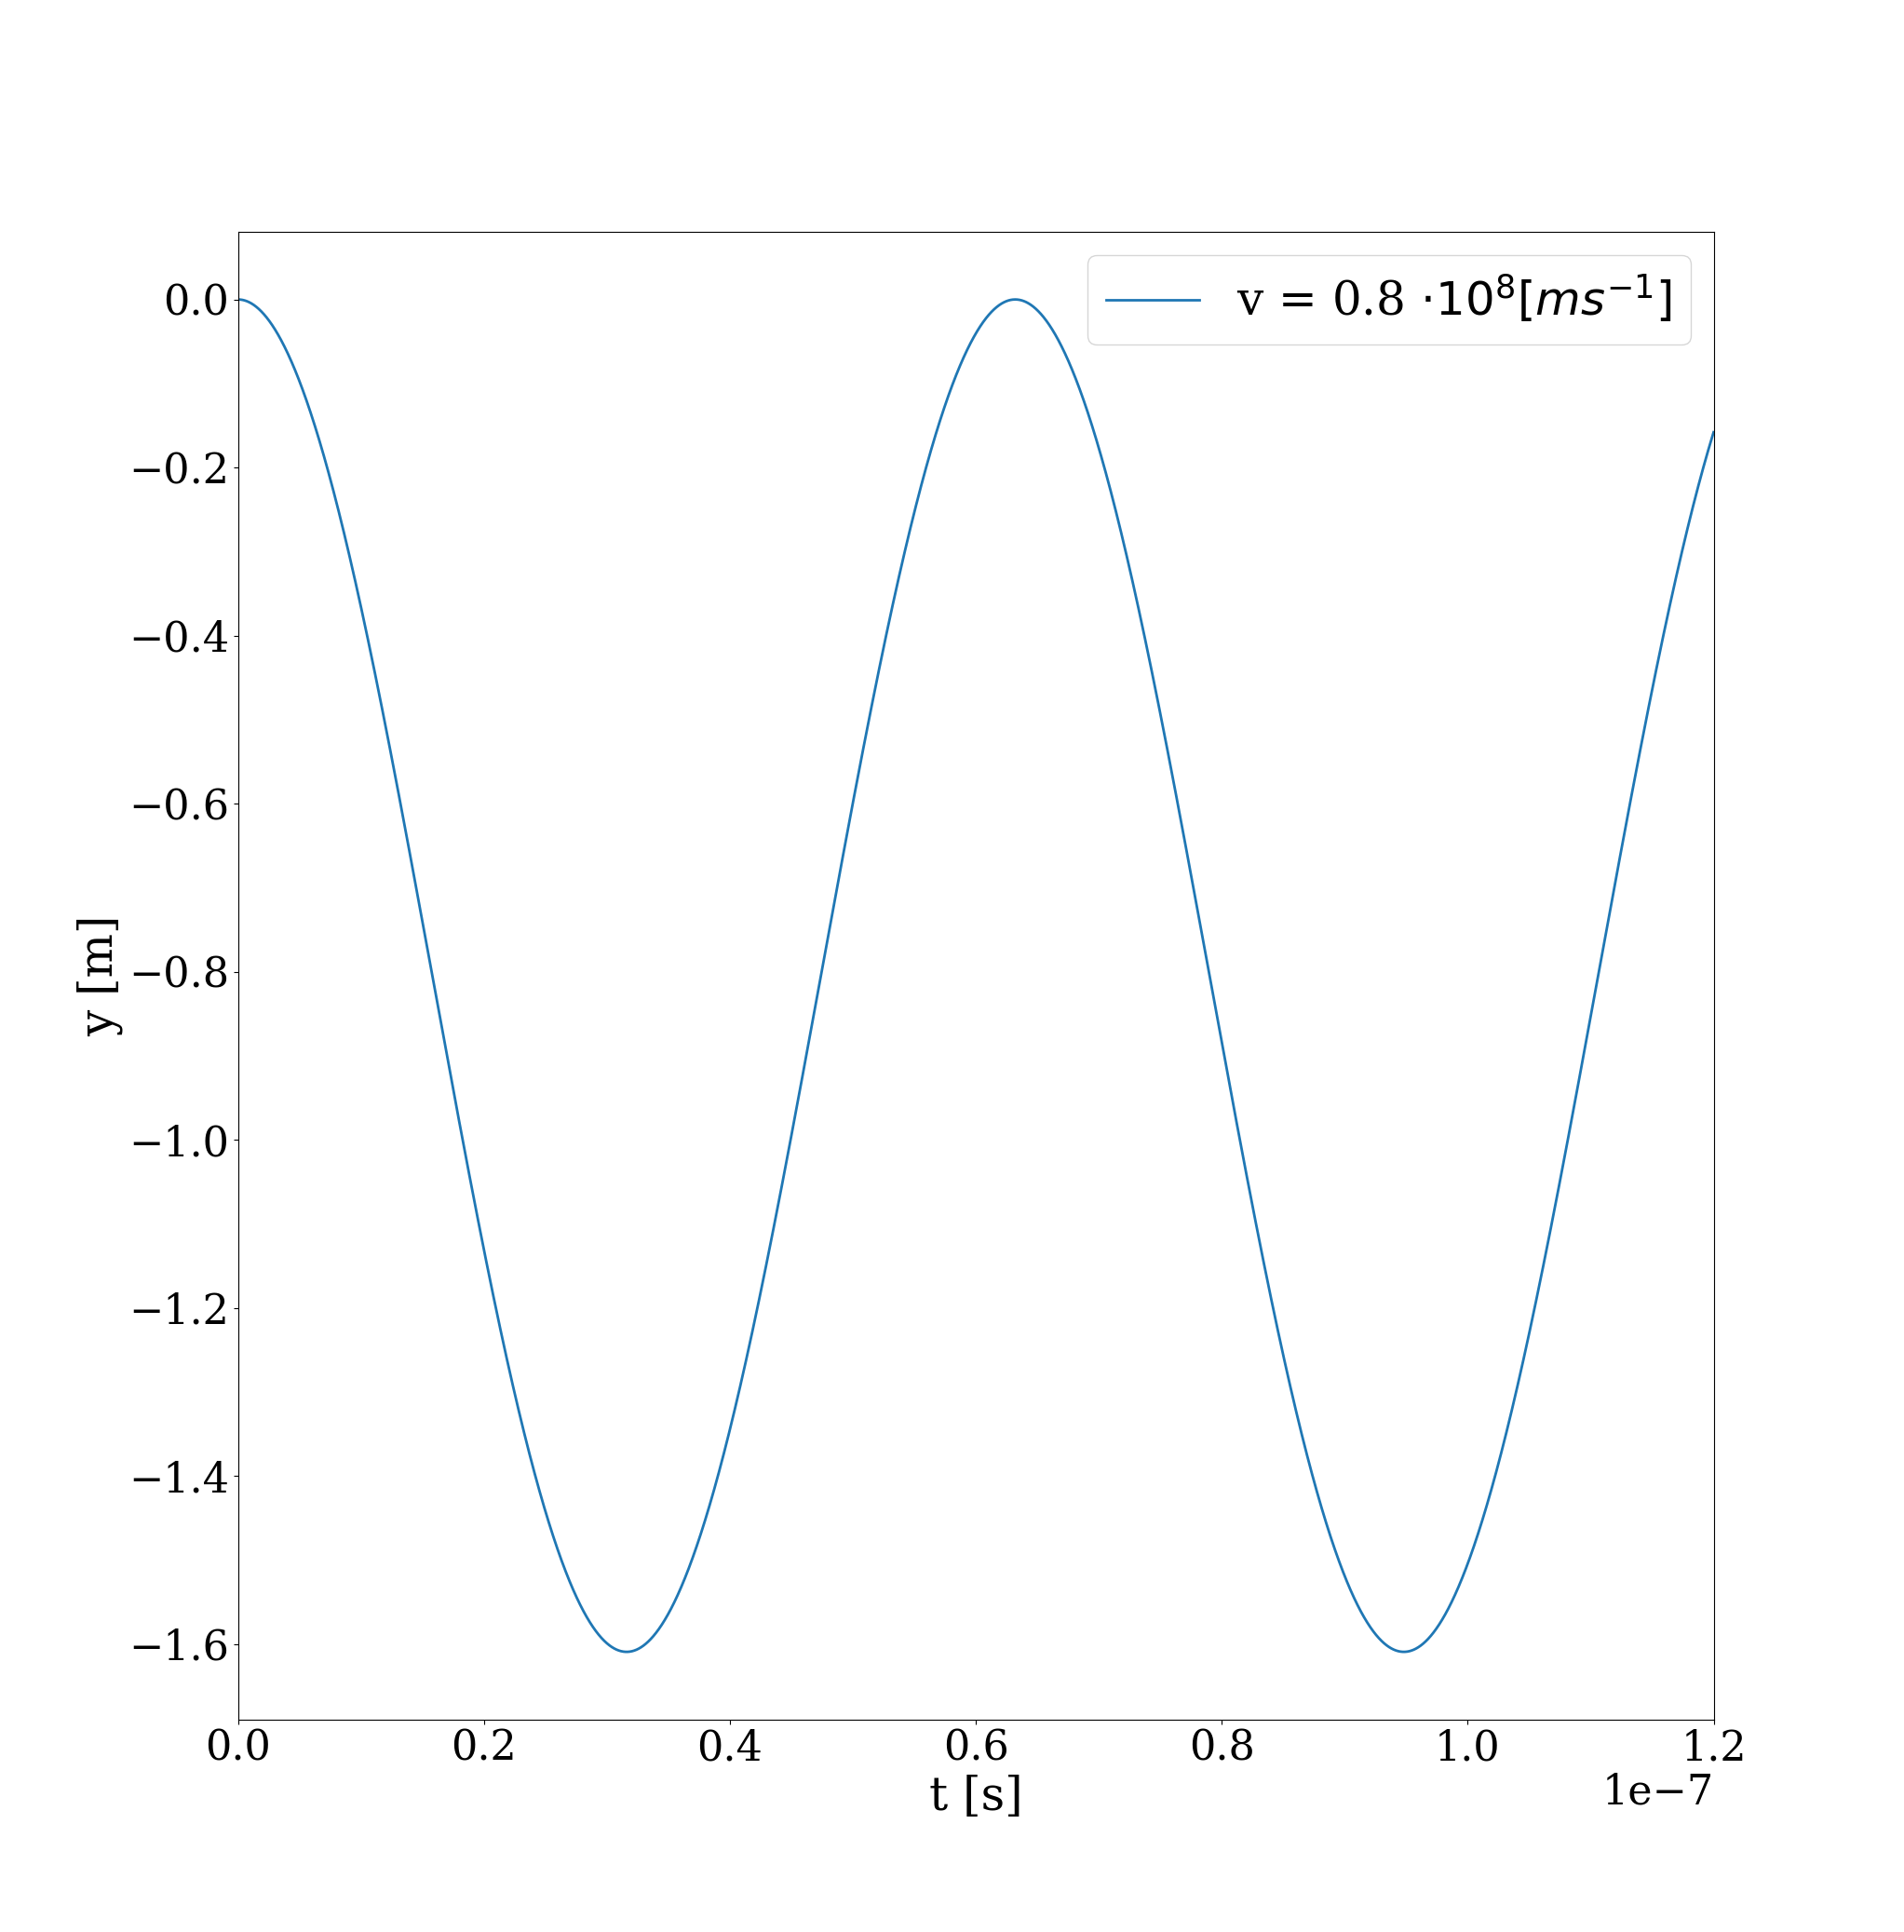
\includegraphics[width=\linewidth]{freq_rel_4.png}
\end{figure}

\begin{figure}
    \centering
    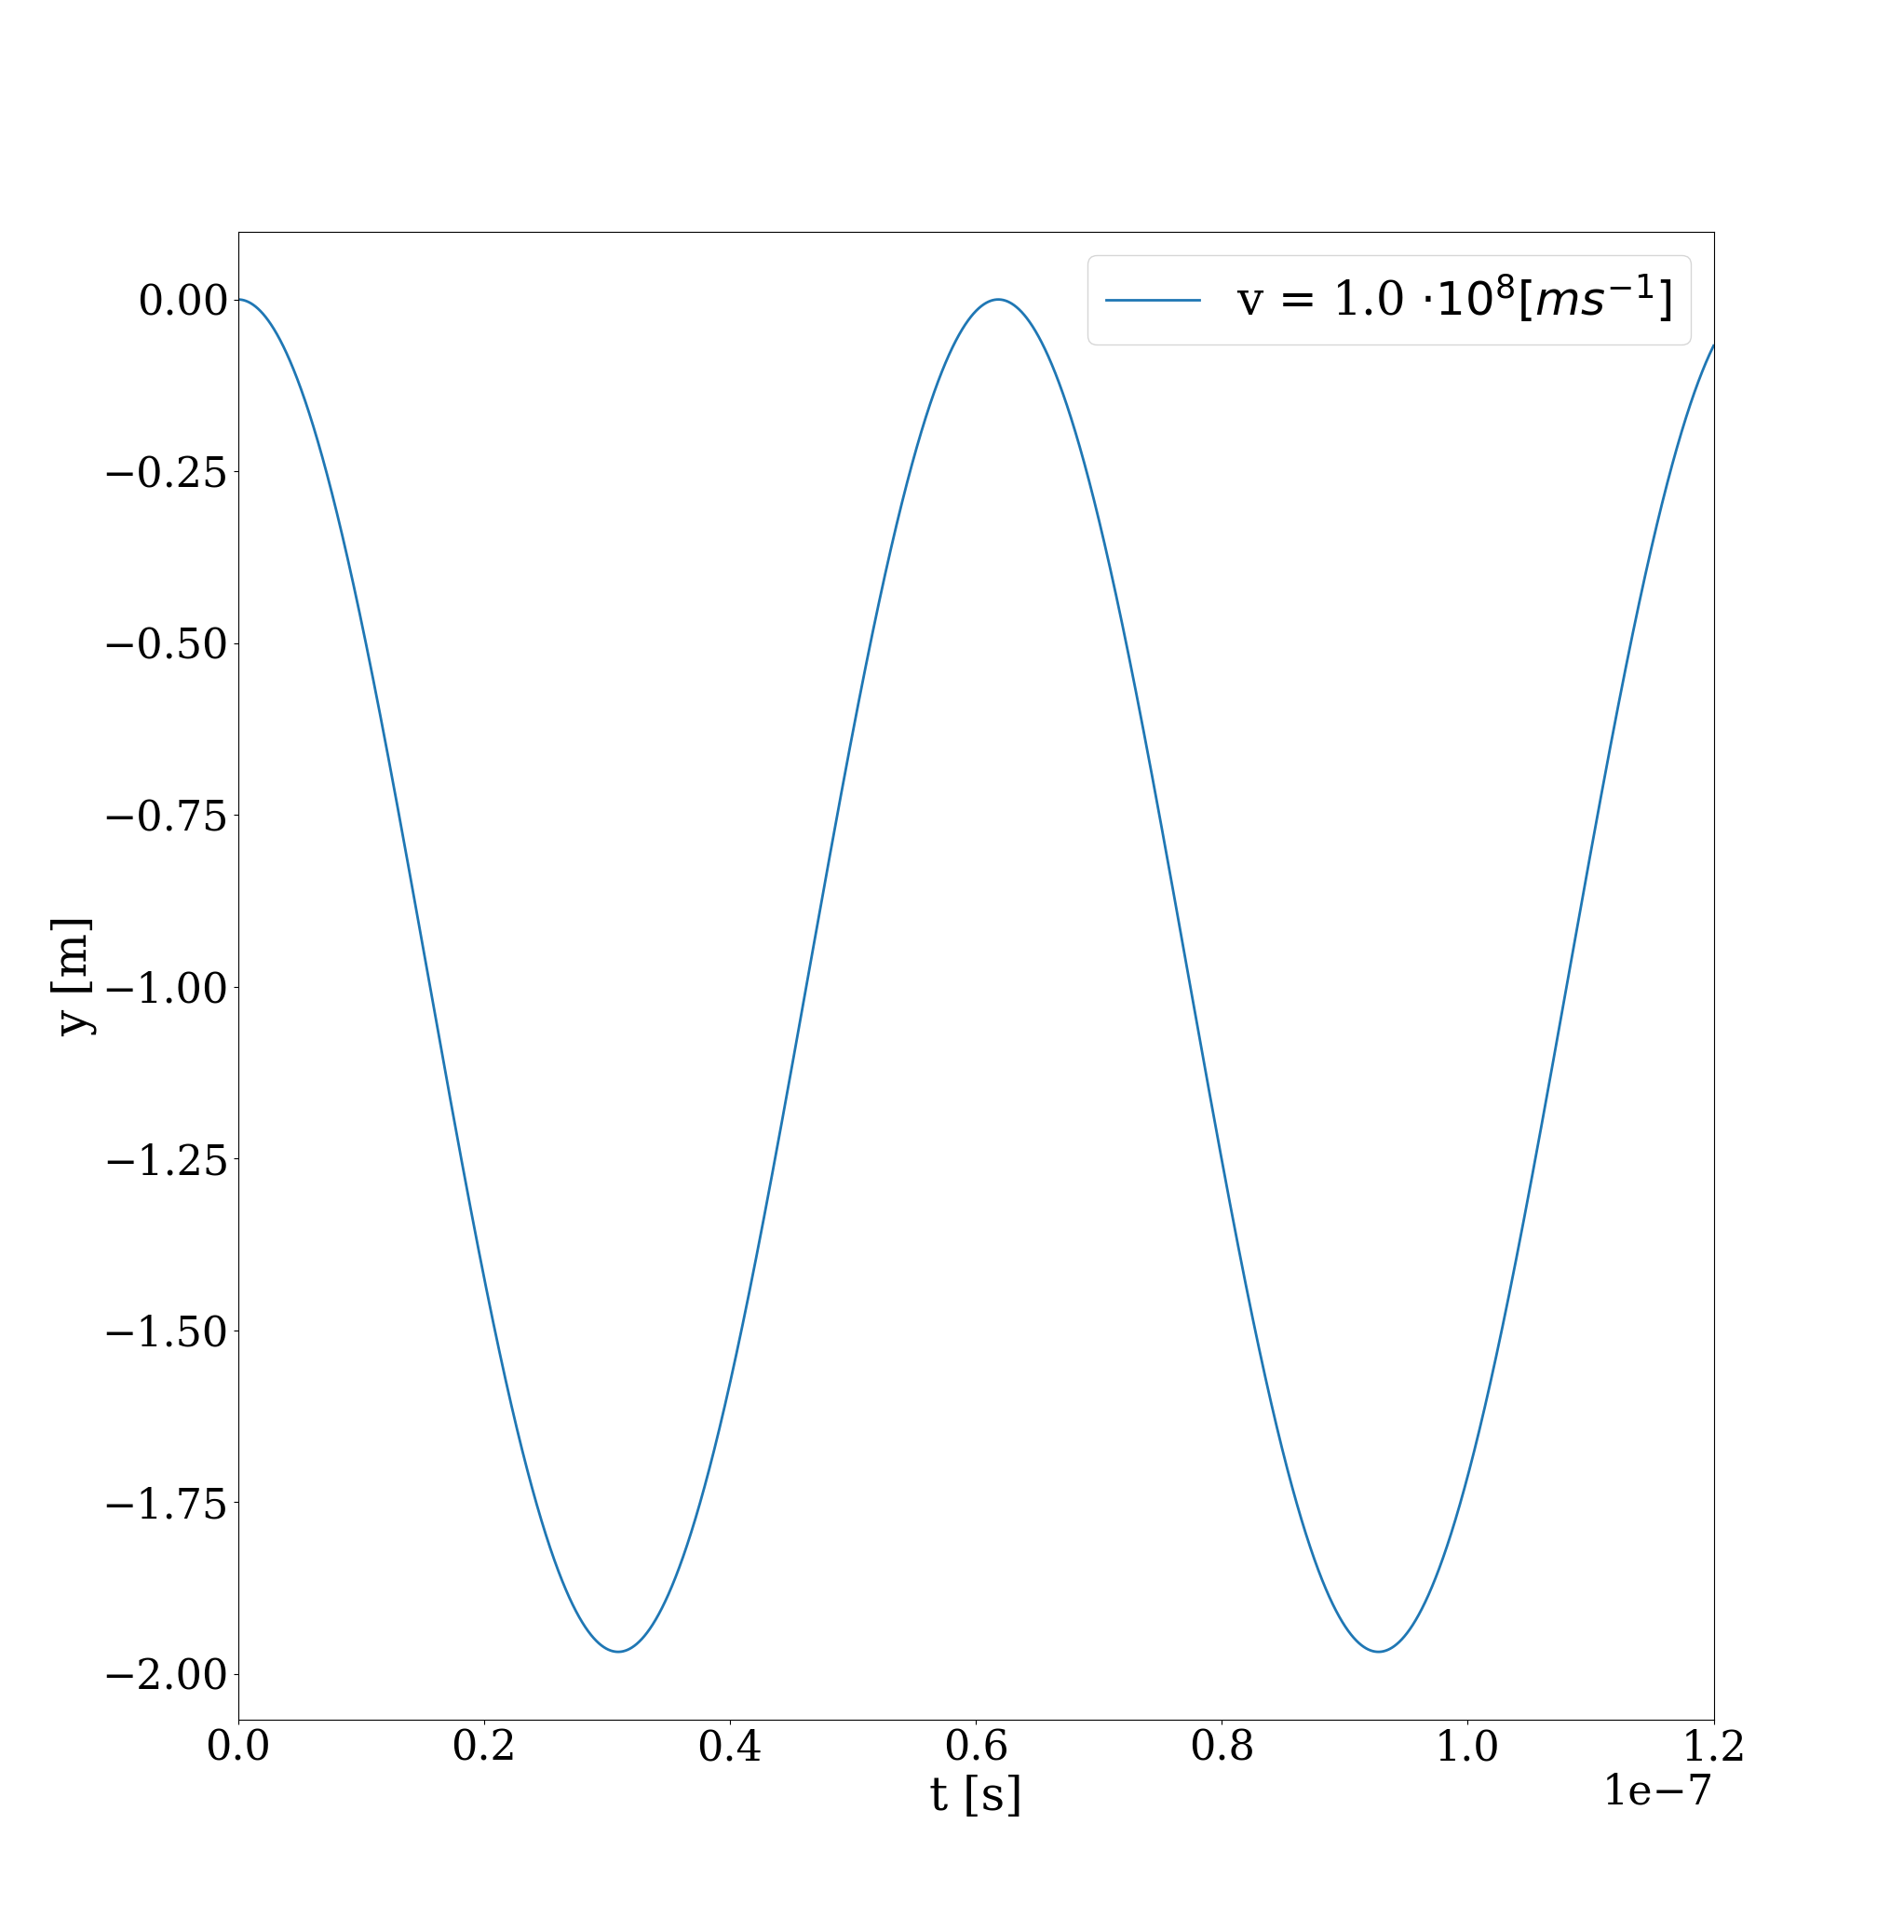
\includegraphics[width=\linewidth]{freq_rel_5.png}
\end{figure}

\begin{figure}
    \centering
    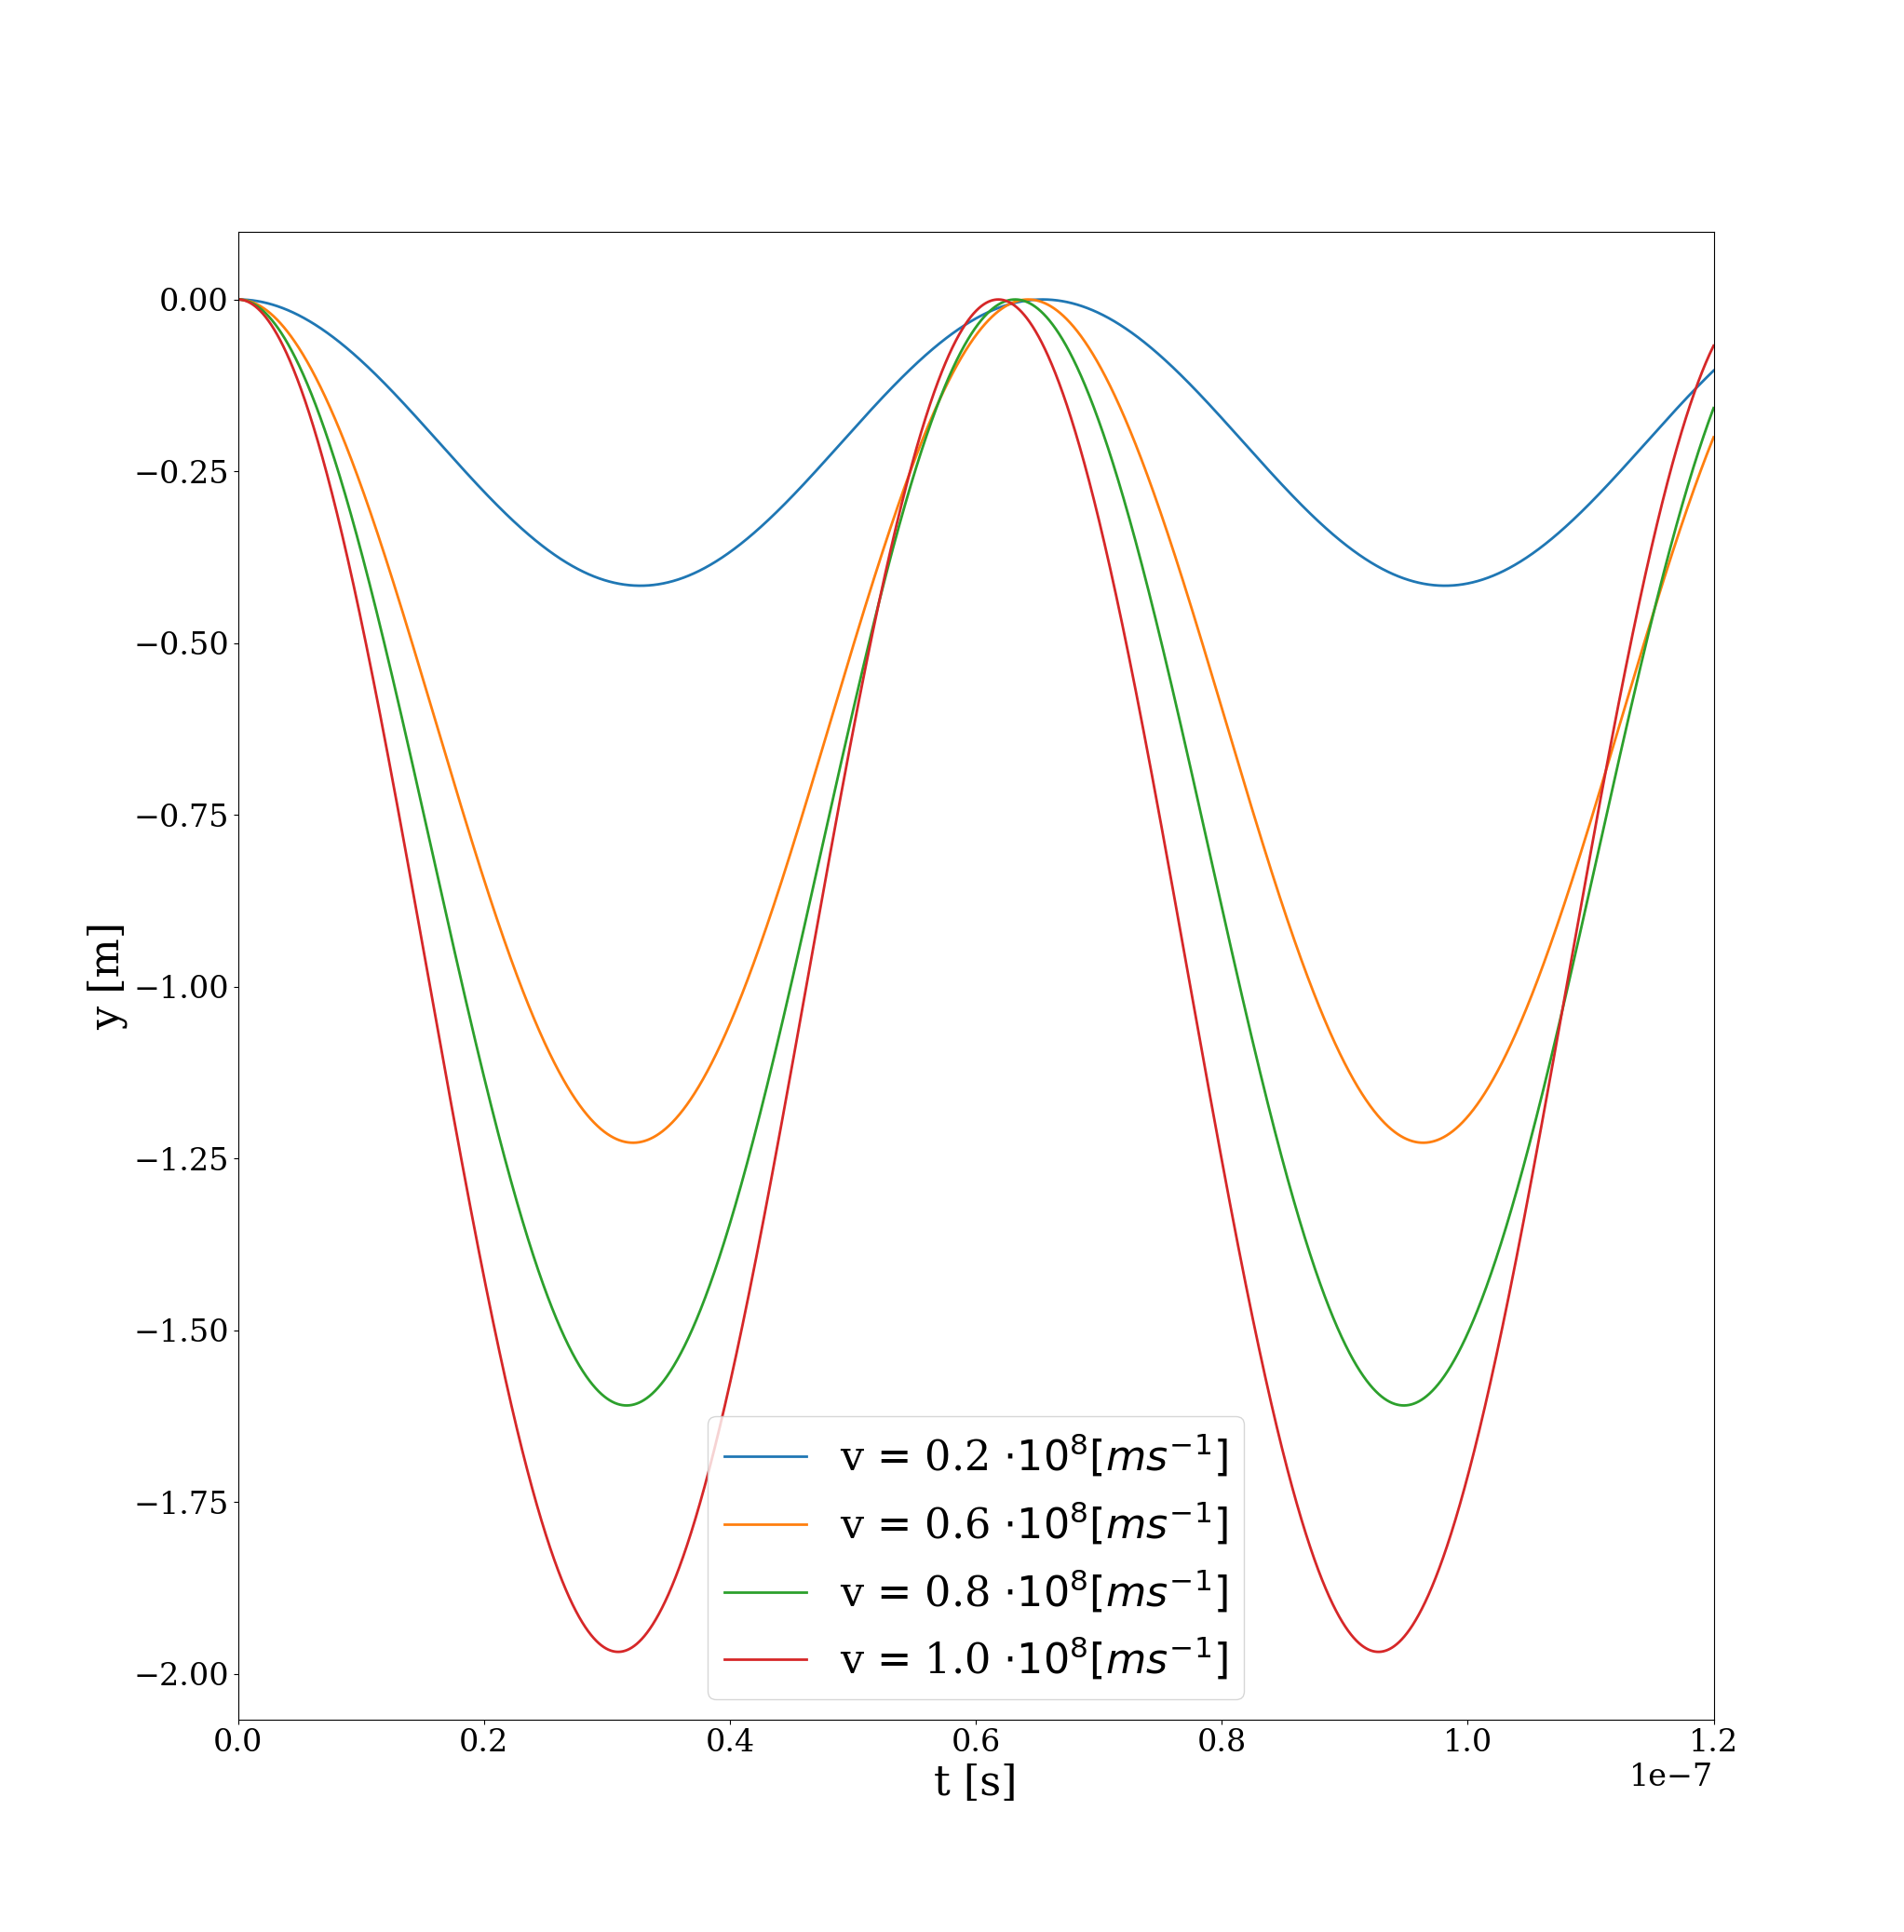
\includegraphics[width=\linewidth]{freq_relativista_relativistas.png}
\end{figure}

\clearpage

\section{Conclusión}
\label{sec:conclusion}


\end{document}
